
\documentclass[a4paper,UKenglish,cleveref, autoref, english, thm-restate]{lipics-v2019}
%This is a template for producing LIPIcs articles. 
%See lipics-manual.pdf for further information.
%for A4 paper format use option "a4paper", for US-letter use option "letterpaper"
%for british hyphenation rules use option "UKenglish", for american hyphenation rules use option "USenglish"
%for section-numbered lemmas etc., use "numberwithinsect"
%for enabling cleveref support, use "cleveref"
%for enabling autoref support, use "autoref"
%for anonymousing the authors (e.g. for double-blind review), add "anonymous"
%for enabling thm-restate support, use "thm-restate"

%\graphicspath{{./graphics/}}%helpful if your graphic files are in another directory

\bibliographystyle{plainurl}% the mandatory bibstyle

\title{Diameter spaces: a partial metric semantics of higher-order programs} %TODO Please add

\titlerunning{A partial metric semantics of higher-order programs  } %TODO optional, please use if title is longer than one line

\author{Guillaume Geoffroy}
{Universit\`a di Bologna, Dipartimento Informatica-Scienza e Ingegneria, Italy}
{guillaume.geoffroy@unibo.it} 
{}
{}

\author{Paolo Pistone}
{Universit\`a di Bologna, Dipartimento Informatica-Scienza e Ingegneria, Italy}
{paolo.pistone2@unibo.it} 
{}
{}
%{johnqpublic@dummyuni.org}{https://orcid.org/0000-0002-1825-0097}{(Optional) author-specific funding acknowledgements}%TODO mandatory, please use full name; only 1 author per \author macro; first two parameters are mandatory, other parameters can be empty. Please provide at least the name of the affiliation and the country. The full address is optional


\authorrunning{G. Geoffroy and P. Pistone} %TODO mandatory. First: Use abbreviated first/middle names. Second (only in severe cases): Use first author plus 'et al.'

\Copyright{G. Geoffroy and P. Pistone} %TODO mandatory, please use full first names. LIPIcs license is "CC-BY";  http://creativecommons.org/licenses/by/3.0/

\ccsdesc[100]{\textcolor{red}{Replace ccsdesc macro with valid one}} %TODO mandatory: Please choose ACM 2012 classifications from https://dl.acm.org/ccs/ccs_flat.cfm 

\keywords{Differential semantics, program metrics, approximate transformations, partial metric spaces} %TODO mandatory; please add comma-separated list of keywords

\category{} %optional, e.g. invited paper

\relatedversion{} %optional, e.g. full version hosted on arXiv, HAL, or other respository/website
%\relatedversion{A full version of the paper is available at \url{...}.}

\supplement{}%optional, e.g. related research data, source code, ... hosted on a repository like zenodo, figshare, GitHub, ...

%\funding{(Optional) general funding statement \dots}%optional, to capture a funding statement, which applies to all authors. Please enter author specific funding statements as fifth argument of the \author macro.

\acknowledgements{I want to thank \dots}%optional

%\nolinenumbers %uncomment to disable line numbering

%\hideLIPIcs  %uncomment to remove references to LIPIcs series (logo, DOI, ...), e.g. when preparing a pre-final version to be uploaded to arXiv or another public repository

%Editor-only macros:: begin (do not touch as author)%%%%%%%%%%%%%%%%%%%%%%%%%%%%%%%%%%
\EventEditors{John Q. Open and Joan R. Access}
\EventNoEds{2}
\EventLongTitle{42nd Conference on Very Important Topics (CVIT 2016)}
\EventShortTitle{CVIT 2016}
\EventAcronym{CVIT}
\EventYear{2016}
\EventDate{December 24--27, 2016}
\EventLocation{Little Whinging, United Kingdom}
\EventLogo{}
\SeriesVolume{42}
\ArticleNo{23}
%%%%%%%%%%%%%%%%%%%%%%%%%%%%%%%%%%%%%%%%%%%%%%%%%%%%%%


%packages


\usepackage{booktabs}   %% For formal tables:
                        %% http://ctan.org/pkg/booktabs
\usepackage{subcaption} %% For complex figures with subfigures/subcaptions
%% http://ctan.org/pkg/subcaption
\usepackage{amsmath, amssymb}
\usepackage{xifthen}
\usepackage{tikz,pgfplots}
\usepackage{stmaryrd}
\usetikzlibrary{cd}

\usepackage{rotating}
\usepackage{comment}
\usepackage{adjustbox}
\usepackage{pgfplots}
\usetikzlibrary{intersections}



\tikzset{commutative diagrams/.cd,
mysymbol/.style={start anchor=center,end anchor=center,draw=none}
}
\newcommand\Lessone[2][\begin{rotate}{25}{\huge$\leq$}\end{rotate}]{%
  \arrow[mysymbol]{#2}[description]{#1}}
\newcommand\Lesstwo[2][\begin{rotate}{25}{\huge$\geq$}\end{rotate}]{%
  \arrow[mysymbol]{#2}[description]{#1}}



%macros


%% Custom command definitions
\newcommand{\ob}[1]{\operatorname{Ob}\left(#1\right)}
\newcommand{\close}[1]{\overline{#1}}
% \newcommand{\intervals}[1]{???}
%\newcommand{\intervalsx}[1]{\left[#1\right]}
%\newcommand{\intervals}[1]{\overline{\left[#1\right]}}
\newcommand{\I}{\mathcal{I}}
\newcommand{\J}{\mathcal{J}}
\newcommand{\K}{\mathcal{K}}
\newcommand{\apcat}{\mathcal{A}}
\newcommand{\apcatT}{\mathcal{A}^{\tang}}
\newcommand{\apcatd}{\mathcal{A}_d}
\newcommand{\pmcat}{\mathcal{M}}
\newcommand{\epcat}{\mathcal{E}}
\newcommand{\diff}{\partial}
\newcommand{\tang}{T}
\newcommand{\pmofap}[1]{\ifthenelse{\isempty{#1}}{\left\vert-\right\vert}{\left\vert#1\right\vert}}
\newcommand{\setcat}{\operatorname{Set}}
\newcommand{\posetcat}{\operatorname{Poset}}
\newcommand{\R}{\mathbb{R}}
\newcommand{\cart}{\times}%{\mathbin{\&}}
\newcommand{\projL}{\pi_1}
\newcommand{\projR}{\pi_2}

\newcommand{\oneap}{1}
\newcommand{\onequantale}{1}

\newcommand{\id}[1][]{\ifthenelse{\isempty{#1}}{\operatorname{id}}{\operatorname{id}_{#1}}}

\newcommand{\ev}{\operatorname{ev}}
\newcommand{\lam}{\lambda}

\newcommand{\dsp}{\operatorname{Diam}}
\newcommand{\bs}[1]{\left\vert#1\right\vert}
\newcommand{\set}{\operatorname{Set}}
\newcommand{\eff}{\operatorname{Eff}}
\newcommand{\scott}{\operatorname{Scott}}

%\newcommand{\oplam}{\operatorname{lam}}

\newcommand{\STLC}{\mathsf{ST\lambda C}(\mathcal F_{n})}
\newcommand{\QMet}{\mathsf{Met}_Q}
\newcommand{\RMet}{\mathsf{Met}_{\R_+^\infty}}
%\newcommand{\GPMS}{\mathsf{GPMet}}
\newcommand{\gpms}[1]{#1}
\newcommand{\real}{\R}
%\newcommand{\Int}{\mathsf{Int}}
\newcommand{\To}[2]{#1 \Rightarrow #2}
\newcommand{\abs}{\lambda}


\newcommand{\ball}{\mathsf{B}}


\newcommand{\B}[1]{\mathbf{#1}}%{\mathbin{\&}}
\newcommand{\powerset}{\mathcal{P}}

\newcommand{\intervals}[1]{\llbracket #1 \rrbracket}
\newcommand{\distances}[1]{\llparenthesis #1 \rrparenthesis}
\newcommand{\tointerval}[1]{\overline{#1}}
\newcommand{\quantaleleq}{\sqsubseteq}
\newcommand{\quantalegeq}{\sqsupseteq}
\newcommand{\quantaleop}{\mathbin{\ast}}
\newcommand{\diam}{\delta}
\newcommand{\oeq}{\approx}

\newcommand{\metalambda}{%
  \mathop{%
    \rlap{$\lambda$}%
    \mkern2mu
    \raisebox{.275ex}{$\lambda$}%
  }%
}



\begin{document}

\maketitle

%TODO mandatory: add short abstract of the document
\begin{abstract}
Abstract
\end{abstract}


\section{Introduction}

% !TEX root = CSL 2021.tex

%\subparagraph*{Measuring sensitivity and similarity of programs in a compositional way}
In program semantics one is usually interested in capturing notions of behavioral equivalence between programs. However,  sin several fields like approximate \cite{Mittal2016}, incremental \cite{Cai2014, Picallo2019} and probabilistic \cite{10.1109/LICS.2015.64} computation, it is often more useful to be able to describe \emph{to which extent}  two programs behave in a similar, although non equivalent way, so that one can measure the change in the result produced by
replacing one program by the other one.
% produces a change in the result which can be quantified and bounded in some way.



This idea has motivated much literature on program (pseudo)metrics \cite{ARNOLD1980181, VANBREUGEL20011,Azevedo_de_Amorim_2017, Escardo1999, BAIER1994171,10.1109/LICS.2015.64, 10.1007/978-3-662-44584-6_4, 10.1007/978-3-662-54434-1_13, 10.1145/3209108.3209149}, that is, on semantics in which types are endowed with a notion of distance measuring the differences in their behaviors. This approach has found widespread applications, for example in differential privacy \cite{10.1145/1932681.1863568, 10.1007/978-3-642-29420-4_3, Barthe_2012}, where one is interested in measuring the \emph{sensitivity} of a program, \textit{i.e.} its capacity to amplify changes in its inputs, and in the study of probabilistic processes \cite{DESHARNAIS2004323, VANBREUGEL2005115, 10.1007/978-3-662-44584-6_4,10.1007/3-540-48224-5_35}.


Recent literature \cite{chaudhuri, dallago:differential-stlc} has highlighted the importance of \emph{contextuality} to reason about program similarity: many common situations  require to measure the error produced by a transformation of the form $\mathtt C[t] \leadsto \mathtt C[u]$, which replaces a program $t$ by $u$ \emph{within a context} $\mathtt C[\ ]$, as a function of the mismatch between $t$ and $u$ and of the sensitivity of the context $\mathtt C[\ ]$ itself.
 For instance, the error produced by replacing the program $\lambda x.\sin(x)$ by the identity function $\lambda x.x$
  in a given context  $\mathtt C$ will 
  be highly sensitive to how close to $0$  
  these functions are evaluated in $\mathtt C$.
 Similar cases of contextual reasoning can be found  in many areas of computer science: for example 
 in techniques from numerical analysis (\emph{e.g.}~the Gauss-Newton method), in which a 
 computationally intensive function is replaced by its Taylor's expansion {around some given point}, or in {approximate computing} techniques like \emph{loop perforation} \cite{loopperf}, in which a compiler can be asked to skip a certain number of iterations of a loop in a program.

\subparagraph*{The Problem of Coupling Program Metrics with Higher-Order Types}

\begin{figure}
\begin{subfigure}{0.48\textwidth}
\parbox[h][3.5cm][c]{\textwidth}{
\adjustbox{center}{$
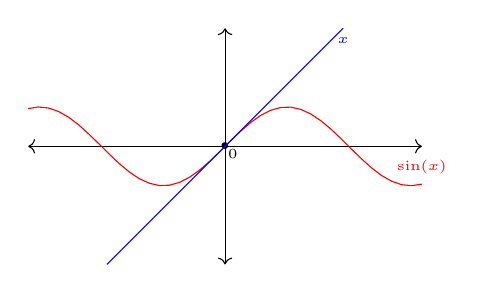
\begin{tikzpicture}[domain=-5:5, scale=0.5]
%\draw[very thin,color=gray] (-0.1,-1.1) grid (3.9,3.9);
\draw[<->]   (-5,0) -- (5,0);
\draw[<->] (0,-3) -- (0,3); % node[above] {$f(x)$};

   \node at (0.2,-0.2){\tiny$0$};
      \node at (0,0){\tiny$\bullet$};

%
\draw[color=red, domain=-5:5, samples=40] plot (\x, {sin(\x r)} ) node[above] {\tiny$\sin(x)$};

\draw[color=blue, domain=-3:3, samples=40] plot (\x,{\x  } ) node[below] {\tiny$x$};


\end{tikzpicture}$}
}
\caption{\small $\sin(x)$ and $x$ are very close around $0$, but their distance diverges at $\pm \infty$.}
\label{fig:sinid1}
\end{subfigure} \ \ \ 
\begin{subfigure}{0.48\textwidth}
\parbox[h][3.5cm][c]{\textwidth}{
\adjustbox{center}{$
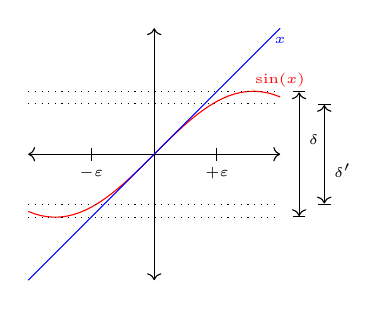
\begin{tikzpicture}[domain=-2:2, scale=0.8]
%\draw[very thin,color=gray] (-0.1,-1.1) grid (3.9,3.9);
\draw[<->]   (-2,0) -- (2,0);
\draw[<->] (0,-2) -- (0,2); % node[above] {$f(x)$};


\draw[|-|] (-1,0) -- (1,0);
\node(r) at (-1,-0.3) {\tiny$-\varepsilon$};
\node(r) at (1,-0.3) {\tiny$+\varepsilon$};
   % \node at (0,0)[circle,fill,inner sep=1pt]{};
%
\draw[color=red, domain=-2:2, samples=40] plot (\x, {sin(\x r) } ) node[above] {\tiny$\sin(x)$};

\draw[color=blue, domain=-2:2,samples=40] plot (\x,{\x  } ) node[below] {\tiny$x$};


\draw[dotted] (-2,1) -- (2,1);
\draw[dotted] (-2,-1) -- (2,-1);

\draw[dotted] (-2,0.8) -- (2,0.8);
\draw[dotted] (-2,-0.8) -- (2,-0.8);

\draw[|<->|] (2.3,1) -- node[above right]{\tiny$\delta$} (2.3,-1);
\draw[|<->|] (2.7,0.8) -- node[below right]{\tiny$\delta'$} (2.7,-0.8);


\end{tikzpicture}$}
}
\caption{\small The self-distances $\delta,\delta'$ of $\sin(x)$ and $x$ in a small interval $[-\varepsilon,\varepsilon]$ of $0$ are very close.}
\label{fig:sinid2}
\end{subfigure}
\caption{The sup-distance is inadequate for contextual transformations.}
\label{fig:sinid}
\end{figure}
 
While several frameworks  for contextual reasoning have been developed in recent years \cite{10.1145/1932681.1863568,Gaboardi_2013,Azevedo_de_Amorim_2017,chaudhuri, dallago:differential-stlc}, these approaches suggest that describing program similarity for a fully higher-order language in terms of program metrics still constitutes a major challenge. 

In particular, when considering higher-order languages with a type $\mathsf{Real}$ for real numbers, it is not clear how to \emph{lift} the standard metric on $\mathsf{Real}$  
 to higher-order types, \emph{e.g.}~to $\mathsf{Real}\to \mathsf{Real}$, so that the distances between higher-order programs are measured in a contextual way.



A standard solution is to take the sup-distance, that is, to let, for $f,g:\mathsf{Real}\to \mathsf{Real}$, $d(f,g)=\sup\{d(f(r),g(r))\mid r\in \mathsf{Real}\}$. This solution works well in models in which programs are interpreted as \emph{non-expansive} or \emph{Lipschitz-continuous} maps \cite{Hofmann2014, Azevedo_de_Amorim_2017}. However such models are not \emph{cartesian-closed}\footnote{In fact, cartesian closed categories of metric spaces and non-expansive functions \emph{do} exist \cite{Escardo1999, Stubbe2009}, but, to our knowledge, none of these categories contains the real numbers with the standard metric.}, so they do not account for 
 the simply-typed lambda-calculus in its full generality, but only for linear or sub-exponential variations of it (such as $\mathsf{Fuzz}$ \cite{10.1145/1932681.1863568,Gaboardi_2013,Azevedo_de_Amorim_2017}).
 Also, it has been shown \cite{10.1109/LICS.2015.64} that in a probabilistic setting the non-linearity of higher-order programs has the effect of \emph{trivialising} metrics, that is, of forcing distances to be either $0$ or $1$, hence collapsing program distances onto usual notions of program equivalence.
Most importantly, even if one restricts to a sub-exponential language, the sup-distance is inadequate to account for contextual transformations as the replacement of $\lambda x.\sin(x)$ by $\lambda x.x$ around $0$, as the sup-distance between these two programs is infinite (see Fig. \ref{fig:sinid}). 
 
 
On the other side of the coin, other approaches like \cite{chaudhuri, dallago:differential-stlc} are fully contextual and higher-order, but provide, at best, only weak approximations of a standard notion of metric.  
 Nonetheless, these approaches introduce the idea, which we retain here, that program differences must be taken as being themselves some kind of programs, relating errors in input with errors in  output, and that accordingly, programs should be split in two different classes: \emph{exact} programs, computing mappings from well-defined inputs to well-defined outputs, and \emph{approximate} programs, mapping errors in the input to errors in the output.


\subparagraph*{Diameter Spaces}

In this paper we introduce a new semantic framework to reason about program similarity and approximate program transformations based on 
a class of higher-order denotational models that we call \emph{diameter space models}. Compared to existing higher-order frameworks, the main novelty of these models is that program similarities are measured by associating each simple type with 
 a \emph{generalized partial metric space}, yielding a lifting of the standard metric on $\mathsf{Real}$ to higher-order types.

Generalized partial metric spaces are a well-investigated class of metric spaces that has been widely applied in program semantics \cite{bkmp:partial-metrics, Bukatin1997, doi:10.1111/j.1749-6632.1994.tb44144.x, Schellekens2004, Samet:2013aa, Stubbe2018, HE201999}. 
Such spaces generalize standard metric spaces in that distances
need not be real numbers, but can be functions or any other type of object that lives in a suitable \emph{quantale} \cite{Hofmann2014}, and \emph{self-distances} $d(x,x)$ need not be $0$ (which leads to a stronger triangular inequality: $d(x,y) + d(z,z)\leq d(x,z)+d(z,y)$).


In our models a higher-order type $A$ is interpreted as a 4-tuple $(|A|, \intervals{A}, \distances{A}, \diam_{A})$ called a \emph{diameter space}, where $|A|$ is a set of \emph{exact} values, $\intervals{A}\subset \mathcal P(|A|)$ is a complete lattice of \emph{approximate} values, $\distances{A}$ is a {quantale}, and $\diam_{A}: \intervals{A}\to \distances{A}$ is a function, called \emph{diameter}, which provides a quantitative measure of approximate values.
The map $\diam_{A}$ generalizes some properties of the diameter function of the standard metric on real numbers. In particular, just like the distance between two real numbers can be described as the diameter of the smallest interval containing them, the map $\diam_{A}$ yields a generalized partial metric  $d_{A}:|A|\times |A|\to \distances{A}$ in which the distance between two exact values of $A$ is measured as the diameter of the smallest approximate value containing them, i.e.  $d_{A}(x,y)=\diam_{A}(x\vee y)$. 


\subparagraph*{New Ways of Measuring Distances between Programs of Functional Type}
% measure distances on $\mathsf{Real}\to\mathsf{Real}$}\varepsilon

In our model, while the distance between two real numbers is measured with the standard metrics (and thus lives in the quantale $[0,\infty]$), the distance between  two programs $f,g:\mathsf{Real}\to \mathsf{Real}$ lives in the functional quantale of monotone maps from \emph{approximate values} of $\mathsf{Real}$ (\emph{i.e.} closed intervals) to positive reals. This function maps a closed interval $a$ to the diameter of the smallest interval containing \emph{both} $f(a)$ and $g(a)$. 
Note that, with this definition, 
 the distance of $f$ \emph{from itself}, which needs not be (constantly) 0,  provides a measure of the sensitivity of $f$, since it associates each interval $a$ with the size of the interval $f(a)$ spanned by $f$ on $a$. 
 

The use of partial metrics with functional distances yields a rich and expressive framework to reason about  
contextual transformations. For instance, we can express the closeness of $\lambda x.\sin(x)$ and $\lambda x.x$ around 0 by the fact that their distance, applied to a small interval $[-\varepsilon,\varepsilon]$ around 0, is very close to the {self-distance} of
$\lambda x.\sin(x)$ on the same interval (as illustrated in Fig. \ref{fig:sinid2}). Moreover, the {triangular inequality} of partial metrics  can be used to infer new bounds from previously established ones in a compositional way.


\begin{figure}
\begin{subfigure}{0.45\textwidth}
\parbox[h][4.6cm][c]{\textwidth}{
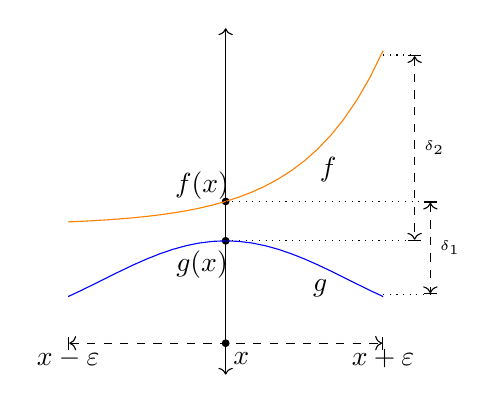
\begin{tikzpicture}[domain=-2:2]
%\draw[very thin,color=gray] (-0.1,-1.1) grid (3.9,3.9);
\draw[dashed, |<->|]   (-2,0) -- (2,0);
\draw[<->] (0,-0.4) -- (0,4); % node[above] {$f(x)$};

    \node at (0,0)[circle,fill,inner sep=1pt]{};
%    \node at (-2,0)[circle,fill,inner sep=1pt]{};
%    \node at (2,0)[circle,fill,inner sep=1pt]{};
\node(z) at (0.2,-0.2) {$x$};
\node(-e) at (-2,-0.2) {$x-\varepsilon$};
\node(e) at (2,-0.2) {$x+\varepsilon$};


\node(f) at (0,0.8+0.5)[circle,fill,inner sep=1pt]{};
\node(f) at (0,1.5+0.3)[circle,fill,inner sep=1pt]{};

\node(f) at (-0.3,2) {$f(x)$};

\node(f) at (-0.3,1) {$g(x)$};


\node(ff) at (1.3,2.2) {{$f$}};
\node(gg) at (1.2,0.7) {{$g$}};

%\draw[color=red] plot (\x,\x) node[right] {$f(x) =x$};
% \x r means to convert ?\x? from degrees to _r_adians:
\draw[color=blue] plot (\x,{0.8+ 0.5*(cos(\x r))}) ;
\draw[color=orange] plot (\x,{1.5+0.3*exp(\x)}) ;

\draw[dotted] (0,1.8) -- (2.6,1.8);
\draw[dotted] (2,0.62) -- (2.6,0.62);
\draw[dotted] (0,1.3) -- (2.4,1.3);
\draw[dotted] (2,3.66) -- (2.4,3.66);

%
%\draw[dotted] (0,1.8) -- (2, 0.62);
%\draw[dotted] (0,1.3) -- (2, 3.66);

\draw[dashed,|<->| ] (2.4,3.66) -- node[right] {\tiny$\delta_{2}$} (2.4,1.3);
\draw[dashed,|<->| ] (2.6,1.8) -- node[right] {\tiny$\delta_{1}$} (2.6,0.62);

\end{tikzpicture}
}
\caption{\small In differential logical relations the distance between two functions $f,g:\R\to \R$, computed at $(x,\varepsilon)$ is the maximum between 
$\delta_{1}=\max\{d(f(x),g(y));~ y\in [x-\varepsilon, x+\varepsilon]\}$ and 
$\delta_{2}=\max\{d(g(x), f(y));~ y\in [x-\varepsilon, x+\varepsilon]\}$.}
% and 
%
%
%minimum $\delta$ such that for all $y\in [x-\varepsilon, x+\varepsilon]$, both $g(y)\in [f(x)-\delta, f(x)+\delta]$ and $f(y)\in[g(x)-\delta, g(x)+\delta]$ hold. $\delta$ is thus $\max\{\delta_{1},\delta_{2}\}$ in the image above.}
\label{fig:graph1}
\end{subfigure} \ \ \ \ 
\begin{subfigure}{0.45\textwidth}
\parbox[h][4.6cm][c]{\textwidth}{
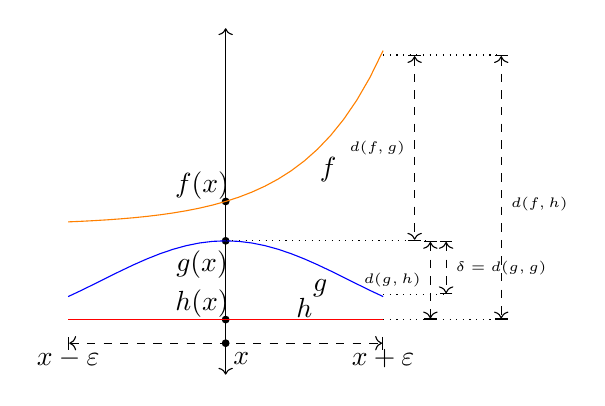
\begin{tikzpicture}[domain=-2:2]
%\draw[very thin,color=gray] (-0.1,-1.1) grid (3.9,3.9);
\draw[dashed, |<->|]   (-2,0) -- (2,0);
\draw[<->] (0,-0.4) -- (0,4); % node[above] {$f(x)$};

    \node at (0,0)[circle,fill,inner sep=1pt]{};
%    \node at (-2,0)[circle,fill,inner sep=1pt]{};
%    \node at (2,0)[circle,fill,inner sep=1pt]{};
\node(z) at (0.2,-0.2) {$x$};
\node(-e) at (-2,-0.2) {$x-\varepsilon$};
\node(e) at (2,-0.2) {$x+\varepsilon$};


\node(f) at (0,0.8+0.5)[circle,fill,inner sep=1pt]{};
\node(f) at (0,1.5+0.3)[circle,fill,inner sep=1pt]{};
\node(f) at (0,0.3)[circle,fill,inner sep=1pt]{};

\node(f) at (-0.3,2) {$f(x)$};

\node(f) at (-0.3,1) {$g(x)$};

\node(f) at (-0.3,0.5) {$h(x)$};

\node(ff) at (1.3,2.2) {{$f$}};
\node(gg) at (1.2,0.7) {{$g$}};
\node(gg) at (1,0.45) {{$h$}};

%\draw[color=red] plot (\x,\x) node[right] {$f(x) =x$};
% \x r means to convert ?\x? from degrees to _r_adians:
\draw[color=blue] plot (\x,{0.8+ 0.5*(cos(\x r))}) ;
\draw[color=orange] plot (\x,{1.5+0.3*exp(\x)}) ;
\draw[color=red] plot (\x,{0.3}) ;



\draw[dotted] (0,1.3) -- (2.6,1.3);
\draw[dotted] (2,0.3) -- (3.5,0.3);
\draw[dotted] (0,1.3) -- (2.4,1.3);
\draw[dotted] (2,3.66) -- (3.5,3.66);
\draw[dotted] (2,0.62) -- (2.8,0.62);

%
%\draw[dotted] (0,1.8) -- (2, 0.62);
%\draw[dotted] (0,1.3) -- (2, 3.66);

\draw[dashed,|<->| ] (2.4,3.66) -- node[left] {\tiny$d(f,g)$} (2.4,1.3);
\draw[dashed,|<->| ] (2.6,1.3) -- node[left] {\tiny$d(g,h)$} (2.6,0.3);

\draw[dashed,|<->| ] (2.8,1.3) -- node[right] {\tiny$\delta=d(g,g)$} (2.8,0.62);

%\draw[dashed,|<->| ] (3.5,2.96) -- node[above right] {\tiny$\begin{matrix}d(f,g)+d(g,h)\\ -d(g,g)\end{matrix}$} (3.5,0.3);

\draw[dashed,|<->| ] (3.5,3.66) -- node[below right] {\tiny$d(f,h)$} (3.5,0.3);

\end{tikzpicture}
}
%
\caption{\small The distance arising from differential logical relations is not a partial metric: the example above shows that $d(f,h)> d(f,g)+d(g,h)- d(g,g)$ (with all distances computed at $(x,\varepsilon)$).}% and 
%
%
%minimum $\delta$ such that for all $y\in [x-\varepsilon, x+\varepsilon]$, both $g(y)\in [f(x)-\delta, f(x)+\delta]$ and $f(y)\in[g(x)-\delta, g(x)+\delta]$ hold. $\delta$ is thus $\max\{\delta_{1},\delta_{2}\}$ in the image above.}
\label{fig:graph2}
\end{subfigure}
\caption{Differential logical relations do not yield partial metrics.}
\end{figure}

A primary source of inspiration for our approach was the recent work by Dal Lago, Gavazzo and Yoshimizu on  \emph{differential logical relations} \cite{dallago:differential-stlc}. This is a semantical framework for higher-order languages in which a type is interpreted as a set $X$ endowed with a kind of metric structure expressed by a ternary relation $\rho \subseteq X\times Q\times X$, where $Q$ is an arbitrary quantale. To our knowledge, this is the first place were the idea of varying the quantales in which distances are measured is introduced as a key ingredient to obtain a cartesian closed category.

While the relation $\rho$ of a GMS induces a distance function $d_{\rho}(x,y)=\sup\{\varepsilon\mid \rho(x,\varepsilon,y)\}$, this function is not a (partial) metric. We can show this fact with a simple example: in this model the distance between two programs 
 $f,g:\mathsf{Real}\to \mathsf{Real}$ is taken in the quantale of functions from $\R\times \R_{+}^{\infty}$ to $\R_{+}^{\infty}$: intuitively, 
  $d(f,g)$ associates a closed interval $[x-\varepsilon,x+\varepsilon]$ (corresponding to the pair $(x,\varepsilon)$) with the smallest distance $\delta$ such that $[ f(x)-\delta, f(x)+\delta]$ and $[g(x)-\delta,g(x)+\delta]$ both contain the images of $[x-\varepsilon, x+\varepsilon]$ through
 $g$ and $f$ respectively (see Fig. \ref{fig:graph1}). Then, as shown in Fig. \ref{fig:graph2}, by letting $\delta=d(g,g)(x,\varepsilon)$, we have that $d(g,g)$ sends the interval $I=[x-\varepsilon, x+\varepsilon]$ onto the interval $[g(x)-\delta, g(x)+\delta]$, which has diameter $2\delta$, while the image of $I$ has diameter $\delta$, making the triangular law of partial metrics fail. 


\subparagraph*{Diameter Space over a Cartesian Closed Category}

Our approach was devised primarily to account for transformations in higher-order languages designed for real analysis computation (like \emph{e.g.} $\mathsf{Real\ PCF}$ \cite{Edalat:2000aa}). However, diameter spaces can be constructed starting from any higher-order programming language with a reasonable denotational semantics. In fact, for \emph{any} cartesian closed category $\mathbb C$, we can construct a cartesian \emph{lax-}closed category $\dsp(\mathbb C)$, whose morphisms can be seen as approximate versions  of the morphisms of $\mathbb C$. The ``lax'' preservation of the cartesian closed structure reflects the fact that, by composing approximations in a higher-order setting, also their error rates compose (typically, approximating non $\beta$-normal $\lambda$-terms will lead to higher error-rates than approximating their $\beta$-normal forms). 



The generality of our construction shows in particular that our partial metric semantics requires no restrictions (\textit{e.g.} Lipschitz-continuity) on morphisms, and adapts well to the model one starts with: for instance, the category $\dsp(\set)$ contains a partial metric on the set of \emph{all}  set-theoretic functions from $\mathbb R$ to $\mathbb R$, while the categories $\dsp(\eff)$ (where $\eff$ is the \emph{effective topos} \cite{hyland:effective-topos}) and $\dsp(\scott)$ show that our approach scales well to a more computability-minded setting.




\section{Preliminaries?}

Partial metric spaces were introduced as a variant of metric spaces in which self-distances can be non-zero. Extensive litterature exists onthem \cite{bkmp:partial-metrics, doi:10.1111/j.1749-6632.1994.tb44144.x, Samet:2013aa}), and they are related to standard metric spaces and their topology in a very strong way: any partial metric generates a standard metric and many fundamental concepts and results on metric topology (\textit{e.g.} Cauchy sequences, completeness, Banach-fixed point theorem) scale well to partial metric spaces \cite{bkmp:partial-metrics, doi:10.1111/j.1749-6632.1994.tb44144.x}.
\emph{Generalized partial metric spaces}, \textit{i.e.} partial metric spaces over an arbitrary quantale, are well-investigated too \cite{AGT2000,AGT7849}: we quickly recall their definition, along with that of a commutative integral quantale (which is the only kind of quantale we will consider here), as we will use these concepts throughout this paper.

\begin{definition} A \emph{commutative integral quantale} is a triple $(Q, \quantaleop, \quantaleleq)$ where:
\begin{itemize}
\item $(Q, \quantaleleq)$ is a complete lattice,
\item $(Q, \quantaleop)$ is a commutative monoid,
\item $\quantaleop$ commutes with arbitrary $\sup$s,
\item the largest element of $Q$ is neutral for $\quantaleop$.
\end{itemize}
\end{definition}

For example, $([0,\infty], +, \geq)$ is a commutative integral quantale whose largest element is $0$ (notice the reversed ordering). It is straightforward to check that for all commutative integral quantales $Q,R$, the product monoid $Q \times R$ equipped with the product ordering is also a commutative integral quantale. In addition, for all posets $X$, the set of monotonically increasing (respectively, decreasing) functions from $X$ to $Q$, equipped with the pointwise monoid operation and the pointwise ordering, is also a commutative integral quantale. An other example of commutative integral quantale is given by the lattice of ideals of any commutative ring, with the product of ideals as the monoid operation.

\begin{definition} A \emph{generalised partial metric space} is the data of a set $X$, a commutative integral quantale $Q$ and a function $d : X \times X \to Q$ such that: \begin{itemize}
\item for all $x,y \in X$, $d(x,x) \quantalegeq d(x,y)$,
\item for all $x,y \in X$, if $d(x,x) = d(x,y) = d(y,y)$, then $x = y$,
\item for all $x,y \in X$, $d(x,y) = d(y,x)$,
\item for all $x,y,z \in X$, $d(x,z) \quantaleop d(y,y) \quantalegeq d(x,y) \quantaleop d(y,z)$.
\end{itemize}
\end{definition}

For all metric spaces $(X,d)$, $(X, ([0,\infty], +, \geq), d)$ is a generalised partial metric space: notice that the triangular inequality in this definition is the opposite of the usual one, which corresponds to the fact that the quantale ordering on $\mathbb{R}$ is the dual of the usual ordering. For a more telling and somewhat archetypal example, take any set $X$ and consider the set $X^{\leq \omega}$ of all sequences of elements of $X$ indexed by an ordinal less that or equal to $\omega$. For all such sequences $s,t$, let $d(s,t) = 2^{-n} \in [0,\infty]$, where $n$ is the length of the largest common prefix to $s$ and $t$: one can check that $(X^{\leq \omega}, [0,\infty], d)$ is indeed a generalised partial metric space -- in fact, if we interpret the prefixes of a sequence as pieces of partial information, then we have $d(s,s) = d(s,t)$ if and only if $t$ is a refinement of $s$ (\textit{i.e.} if it contains more information), and $d(s,s) = 0$ if and only if $s$ is total (\textit{i.e.} if it cannot be refined).

One can check that for all partial metric spaces $(X, Q, d_X)$ and $(Y, R, d_Y)$, $(X \times Y, Q \times R, d_{X \times Y})$ is a generalised partial metric space, where $d_{X \times Y}((x_1, y_1), (x_2, y_2)) = (d_X(x_1, x_2), d_Y(y_1, y_2))$. However, in general, it is not clear how one should define a partial metric on a function space: Section \ref{subsection:type-gpms} will do this in a particular case.


\section{Intervals and program distances for a simply-typed $\lambda$-calculus with a type of reals}
\label{section:stlc}

% !TEX root = CSL 2021.tex

To illustrate our construction, we start from a relatively concrete example: we consider a simply-typed lambda calculus with a base type and primitives for real numbers, and we follow the plan outlined in the introduction, which yields for each simple type a notion of approximate value, approximate function, diameter and distance between programs. Most definitions are straightforward and intuitive: the interesting, not immediately obvious point is that our construction does yield a \emph{partial metric} on each type.

\emph{Simple types} are defined as follows: $\mathsf{Real}$ is a simple type; if $A$ and $B$ are simple types, then $A \to B$ and $A \times B$ are simple types.
For all $n>0$, we fix a set $\mathcal{F}_n$ of functions from $\mathbb{R}^n$ to $\mathbb{R}$. We consider the usual Curry-style simply-typed $\lambda$-calculus over the types defined above (the left and right projection are denoted by $\pi_L:A\times B \to A$ and  $\pi_R:A\times B \to B$ respectively, and the constructor for pairs by $\left\langle-,-\right\rangle$), enriched with the following constants: for all $r \in \mathbb{R}$, a constant $r:\mathsf{Real}$; for all $n>0$ and all $f\in\mathcal{F}_n$, a constant $f:\mathsf{Real}\to\ldots\to\mathsf{Real}\to\mathsf{Real}$. We call this calculus $\STLC$, and its terms are simply called \emph{terms}. We write $t[x_1 := u_1, \ldots, x_n := u_n]$ to denote the \emph{simultaneous} substitution of $u_1, \ldots, u_n$ for $x_1, \ldots, x_n$ in $t$. For all types $A$, we denote by $\Lambda_A$ the set of closed terms of type $A$. The relation of $\beta$-reduction is enriched with the following rule, extended to all contexts: for all $n>0$, $f\in\mathcal{F}_n$, and $r_1,\ldots,r_n\in\mathbb{R}$, $f r_1 \ldots r_n \to_\beta s$, where $s = f(r_1, \ldots, r_n)$. By standard arguments, this calculus has the properties of subject reduction, confluence and strong normalisation.

In addition to the usual notion of $\beta$-equivalence between terms of $\STLC$, we will exploit also a stronger equivalence: given two closed terms $t,u$ of type $A$,  we say that $t$ and $u$ are \emph{observationally equivalent} and write $t \oeq_A u$ if for all terms $C$ such that $x:A \vdash C : \mathsf{Real}$ is derivable, $C[x:=t]$ is $\beta$-equivalent to $C[x:=u]$ (which amounts to saying that they both $\beta$-reduce to the same real number).  It is clear that observational equivalence is a congruence and that two $\beta$-equivalent terms are always observationally equivalent. The notion of distance we define in the next paragraph will be a generalisation of this notion of equivalence.



\subsection{Approximate Values and Approximate Programs}

The first step of our construction for $\STLC$ is to associate to each simple type $A$ a set $\intervals{A}$ whose elements are certain sets of programs of type $A$ that we call \emph{approximate values of type $A$}. 
A closed term $t\in \Lambda_{A}$ represents a program with return type $A$ and no parameters, so an approximate value can be thought as a specification of a program with return type $A$ and no parameters \emph{up to} a certain degree of error or approximation.

For each simple type $A$, the set of approximate values $\intervals{A}\subseteq \mathcal P(\Lambda_A)$ is defined inductively as follows:
\begin{itemize}
\item $\intervals{\mathsf{Real}} = \{ \{ t \in \Lambda_\mathsf{Real} \mid \exists r \in I, t \to_\beta^* r \} \mid I \subseteq \mathbb{R} \text{ is a compact interval or $\emptyset$ or } \mathbb{R} \}$,
\item $\intervals{A \times B} = \{ a \times b \mid a  \in \intervals{A}, b \in \intervals{B} \}$, where $a \times b = \{ t \in \Lambda_{A \times B} \mid \pi_L t \in a \text{ and } \pi_R t \in b \}$,
\item $\intervals{A \to B} = \{ \{ t \in \Lambda_{A \to B} \mid \forall u \in \Lambda_{A},~ tu \in I(u) \} \mid I : \Lambda_A \to \intervals{B} \}$.
\end{itemize}

The approximate values of type $\mathsf{Real}$ are sets of closed programs of type $\mathsf{Real}$ which essentially coincide with the compact intervals of $\mathbb R$, plus the empty set and $\mathbb{R}$ itself. An approximate value in $\intervals{A\times B}$ is a ``rectangle'' $a \times b$, with $a\in \intervals{A}$ and $b \in \intervals{B}$, while an approximate value in $\intervals{A\to B}$ is uniquely determined by a function 
$I$ from closed terms $u\in \Lambda_{ A}$ to approximate values $I(u)\in \intervals{B}$.

For example, any two terms $t,u\in \Lambda_{\mathsf{Real}}$ with normal forms $q, r\in \mathbb{R}$ induce an approximate value $[t,u]_{\mathsf{Real}}= \{v\in \Lambda_{\mathsf{Real}}\mid  v\to_{\beta}^{*} s \land (q\leq s\leq r \vee q\geq s\geq r)\}$ of type $\mathsf{Real}$. Similarly, any two terms $t,u\in \Lambda_{\mathsf{Real}\to \mathsf{Real}}$ induce an approximate value
$[t,u]_{\mathsf{Real}\to \mathsf{Real}}= \{v\in \Lambda_{\mathsf{Real}\to\mathsf{Real}}\mid  
\forall r \in \Lambda_{\mathsf{Real}} \ vr\in [ tr, ur]_{\mathsf{Real}} 
\}$. For instance, if $t= \lambda x.\sin(x)+1$ and $u=\lambda x.\cos(x)-1$, then 
$[t,u]_{\mathsf{Real}\to \mathsf{Real}}$ contains all closed terms corresponding to maps oscillating between $\sin (x)+1$ and $\cos(x)+1$ (\textit{e.g.} the program $\lambda x. \sin(x+1)$, as illustrated in Fig. \ref{fig:interval1}).

\begin{figure}
%\begin{subfigure}{0.42\textwidth}
\parbox[h][3cm][c]{\textwidth}{
\adjustbox{center}{$
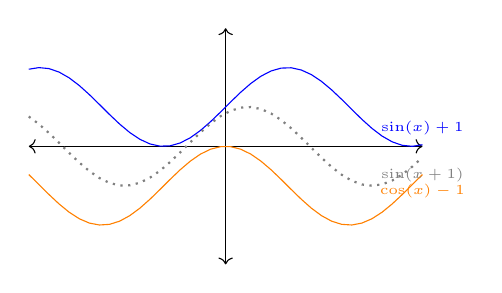
\begin{tikzpicture}[domain=-5:5, scale=0.5]
%\draw[very thin,color=gray] (-0.1,-1.1) grid (3.9,3.9);
\draw[<->]   (-5,0) -- (5,0);
\draw[<->] (0,-3) -- (0,3); % node[above] {$f(x)$};

   % \node at (0,0)[circle,fill,inner sep=1pt]{};
%
\draw[color=blue, samples=40] plot (\x,{sin(\x r)+1}) node[above] {\tiny$\sin(x)+1$};
\draw[color=orange, samples=40] plot (\x,{cos(\x r)-1}) node[below] {\tiny$\cos(x)-1$};

\draw[color=gray, dotted, thick, samples=40] plot (\x,{sin(deg(\x+1) ))}) node[below] {\tiny$\sin(x+1)$};


\end{tikzpicture}$}
}
\caption{$\lambda x.\sin(x+1)$ is in $[\lambda x.\sin(x)+1, \lambda x.\cos(x)+1]_{\mathsf{Real}\to\mathsf{Real}}$.}
\label{fig:interval1}
%\end{subfigure} \ \ \ 
\end{figure}


For all $A$, as a subset of $\mathcal{P}(\Lambda_A)$, $\intervals{A}$ is closed under arbitrary intersections and is therefore a complete lattice whose meet is given by intersection. In particular, for all $t\in\Lambda_A$, there is a least element of $\intervals{A}$ that contains $t$, which will be denoted by $\tointerval{t}$. 
One can check that $\tointerval{t} = \tointerval{u}$ if and only if $t\oeq_{A} u$.

Monotone functions from approximate values to approximate values represent \emph{approximate programs}. They behave like a model of the simply-typed $\lambda$-calculus in a weak sense, namely: \begin{itemize}
\item for all monotone functions $(\alpha_1, \ldots, \alpha_n) \mapsto c[\alpha_1, \ldots, \alpha_n] : \intervals{A_1} \times \ldots \times \intervals {A_n} \to \intervals {B \to C}$ and $(\alpha_1, \ldots, \alpha_n) \mapsto b[\alpha_1, \ldots, \alpha_n] : \intervals{A_1} \times \ldots \times \intervals {A_n} \to \intervals {B}$, we can define a monotone function $(\alpha_1, \ldots, \alpha_n) \mapsto (c[\alpha_1, \ldots, \alpha_n]~ b[\alpha_1, \ldots, \alpha_n]) = \sup\{\tointerval{vu} \mid v \in c[\alpha_1, \ldots, \alpha_n], u \in b[\alpha_1, \ldots, \alpha_n]\} : \intervals{A_1} \times \ldots \times \intervals {A_n} \to \intervals {C}$,
\item for all monotone functions $(\alpha_1, \ldots, \alpha_n) \mapsto c[\alpha_1, \ldots, \alpha_n] : \intervals{A_1} \times \ldots \times \intervals {A_n} \to \intervals {C}$ and all $i \leq n$, we can define a monotone function $(\alpha_j)_{j \neq i} \mapsto (\lambda \alpha_i.~ c[\alpha_1, \ldots, \alpha_n]) = \{ v \in \Lambda_{A_i \to C} \mid \forall t_i \in \Lambda_{A_i},~ v t_i \in c[\alpha_1, \ldots, \tointerval{t_i}, \ldots, \alpha_n] \} : \prod_{j \neq i} \intervals{A_j} \to \intervals{A_i \to C}$,
\end{itemize}
and these two constructions are weakly compatible with $\beta$-reduction and $\eta$-expansion:

\begin{proposition} \label{prop:intervals-weak-model-lambda} For all monotone functions $(\alpha_1, \ldots, \alpha_n, \beta) \mapsto c[\alpha_1, \ldots, \alpha_n, \beta] : \intervals{A_1} \times \ldots \times \intervals {A_n} \times  \intervals {B} \to \intervals {C}$ and $(\alpha_1, \ldots, \alpha_n) \mapsto b[\alpha_1, \ldots, \alpha_n] : \intervals{A_1} \times \ldots \times \intervals {A_n} \to \intervals {B}$, $$\begin{array}{ll} & (\alpha_1, \ldots, \alpha_n) \mapsto (\lambda \beta.~  c[\alpha_1, \ldots, \alpha_n, \beta])~ b[\alpha_1, \ldots, \alpha_n] \\ \leq & (\alpha_1, \ldots, \alpha_n) \mapsto c[\alpha_1, \ldots, \alpha_n, b[\alpha_1, \ldots, \alpha_n]]\text{,}\end{array}$$
and for all monotone functions $(\alpha_1, \ldots, \alpha_n) \mapsto d[\alpha_1, \ldots, \alpha_n] : \intervals{A_1} \times \ldots \times \intervals {A_n} \to  \intervals {B \to C}$,
$$\begin{array}{ll} & (\alpha_1, \ldots, \alpha_n) \mapsto \lambda \beta.~  d[\alpha_1, \ldots, \alpha_n]~ \beta \\ \geq & (\alpha_1, \ldots, \alpha_n) \mapsto d[\alpha_1, \ldots, \alpha_n]\text{,}\end{array}$$
where functions are ordered by pointwise inclusion.  In other words, on approximate programs, $\beta$-reduction and $\eta$-expansion \emph{discard} information, and conversely $\beta$-expansion and $\eta$-reduction \emph{recover} some information.
\end{proposition}

\begin{proof} Without loss of generality, we can assume $n=0$.
Let $v \in \lambda \beta.~ c[\beta]$ and $u \in b$. By definition, $tu \in c[\tointerval{u}]$, so $\tointerval{tu} \subseteq c[\tointerval{u}] \subseteq c[b]$. Therefore, $(\lambda \beta.~ c[\beta])~ b \subseteq b$.
Let $v \in d$. For all $u \in \Lambda_B$, by definition, $vu \in d\tointerval{u}$. Therefore, $v \in \lambda \beta.~ d~ \beta$.
\end{proof}

Beyond theoretical aspects (which will be made clearer in Section 5), 
Proposition \ref{prop:intervals-weak-model-lambda} is also important in practice because it implies that if we compute an approximation of a program from approximations of its parts and then simplify the resulting approximate program using $\beta$-reduction and $\eta$-expansion, what we obtain is still a valid approximation of the original program.


We can define a weak embedding from terms into approximate programs, by mapping each term to its tightest approximation: for all terms $t$ such that $\alpha_{1}:A_{1},\dots,\alpha_{n}:A_{n}\vdash t:B$, we define a monotone function $\partial(t):\intervals{A_{1}}\times \dots \times \intervals{A_{n}} \to \intervals{B}$ by $\partial(t)(a_1, \ldots, a_n) = \sup \{ \tointerval{t u_1 \ldots u_n} \mid u_1 \in \intervals{A_1}, \ldots, u_n \in \intervals{A_n} \}$. 

\begin{remark} \label{remark:push-exp-stlc}
The map $\partial$ is constant on classes of observational equivalence, and one can check that it is is weakly compatible with the constructions of the $\lambda$-calculus, in particular:
\begin{itemize}
\item $\partial (\alpha_{i})(a_{1},\dots, a_{n})=a_{i}$,
\item $\partial (tu)(a_{1},\dots, a_{n}) \subseteq \partial (t)(a_{1},\dots, a_{n}) ~ \partial (u)(a_{1},\dots, a_{n})$,
\item $\partial (\lambda \beta. t)(a_{1},\dots, a_{n}) \subseteq \lambda \beta.~ \partial (t)(\beta, a_{1},\dots, a_{n})$.
\end{itemize}
\end{remark}

This map $\partial(t)$ can be taken as a measure of the \emph{sensitivity} of $t$, as it maps an interval $a$, that is a quantifiably uncertain input, to a quantifiably uncertain output $\partial(t)(a)$. 
For instance, if we take the term $t[x]= \sin(x)+1$ above, then $\partial(t): \intervals{\mathsf{Real}}\to \intervals{\mathsf{Real}}$ sends the interval $[-\pi,\pi]_{\mathsf{Real}}$ into $[0,2]_{\mathsf{Real}}$.

\begin{figure}
%\begin{subfigure}{0.52\textwidth}
\parbox[h][3cm][c]{\textwidth}{
\adjustbox{center}{$
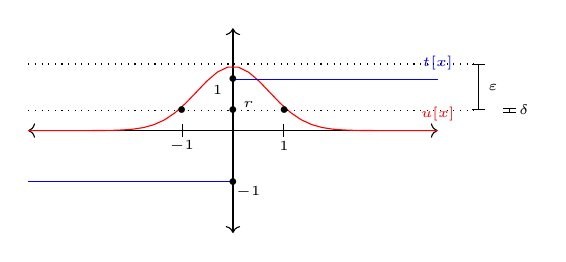
\begin{tikzpicture}[domain=-4:4, scale=0.65]

%\draw[very thin,color=gray] (-0.1,-1.1) grid (3.9,3.9);
\draw[<->]   (-4,0) -- (4,0);
\draw[<->] (0,-2) -- (0,2); % node[above] {$f(x)$};

\draw[dashed, |-|] (-1,0) -- (1,0);
\node(a) at (-1,-0.3) {\tiny$-1$};
\node(a) at (1,-0.3) {\tiny$1$};

\node(a) at (0.3,-1.2) {\tiny$-1$};
\node(a) at (-0.3,0.8) {\tiny$1$};
   % \node at (0,0)[circle,fill,inner sep=1pt]{};

\draw[|-|] (4.8,0.4) -- node[right] {\tiny$\varepsilon$} (4.8,1.3);

\draw[|-|] (5.4,0.35) -- node[right] {\tiny$\delta$} (5.4,0.45);


\draw[color=red, domain=-4:4, samples=40] plot (\x, {(1/2*sqrt(2*pi))*exp(-((\x)^2)) } ) node[above] {\tiny$u[x]$};
%\draw[color=violet, domain=-1.2:1.2] plot (\x, { (\x)^3 } );

\draw[color=blue, domain=-4:0] plot (\x,-1);
\draw[color=blue, domain=0:4] plot (\x,1) node[above] {\tiny$t[x]$};

\draw[dotted] (-4,0.4) -- (4.8,0.4);
\draw[dotted] (-4,1.3) -- (4.8,1.3);

\node(z) at (-1,0.4) {\tiny$\bullet$};
\node(zz) at (1,0.4) {\tiny$\bullet$};

\node(z) at (0,-1) {\tiny$\bullet$};
\node(zz) at (0,1) {\tiny$\bullet$};

\node(r) at (0,0.4) {\tiny$\bullet$};
\node(rr) at (0.3,0.5) {\tiny$r$};



\end{tikzpicture}$}
}
\caption{$\varepsilon=(\partial(u)\circ \partial(t))([-1,1])$ is bigger than $\delta=\partial(u\circ t)([-1,1])=[r,r]$.}
\label{fig:interval2}
%\end{subfigure}
\end{figure}

\begin{remark} \label{remark:oplax-functor-stlc}
When composing two maps $\partial(t)$ and $\partial(u)$, we might obtain a worse approximation than by computing $\partial(t[u/x])$ directly.
For instance, let $t[x]$ and 
$u[x]$ be, respectively, the discontinuous and Gaussian functions illustrated in Fig. \ref{fig:interval2}.  
If $a$ is the interval $[-1,+1]$, then $\partial(t)(a)=[-1,1]$, and since $u[x:=-1]=u[x:=1]\simeq_{\beta} r$ for some $0<r<1$, we deduce that $\partial(u)(\partial(t)(a))=[-1,1] \supsetneq [r,r  ]= \partial (u[t/x])(a)$.

\end{remark}










\subsection{A Partial Metric on Each Type}
\label{subsection:type-gpms}

We will now show how to associate to each type $A$ of $\STLC$ a generalised partial metric space $(\Lambda_{A}/\oeq_{A}, \distances{A}, d_{A})$. The definition of this space will exploit in an essential way the sets of approximate values $\intervals{A}$.


For all simple types $A$, we define a commutative integral quantale $(\distances{A}, \quantaleleq_A, \quantaleop_A)$ of \emph{distances of type $A$}:
\begin{itemize}
\item $(\distances{\mathsf{Real}}, \quantaleleq_\mathsf{Real}, \quantaleop_\mathsf{Real}) = ([0,\infty], \geq, +)$,
\item $\distances{A \times B} = \distances{A} \times \distances{B}$,
\item $\distances{A \to B} = \{ \text{monotonically decreasing functions from } \intervals{A} \text{ to } \distances{B} \}$.
\end{itemize}

Observe that the quantale $\distances{A\to B}$ is a set of functions over the approximate values of $A$.
For all simple types $A$, we now define a \emph{distance function} $d_A : \Lambda_A \times \Lambda_A \to \distances{A}$:
\begin{itemize}
\item $d_\mathsf{Real}(t,u) = \left\vert r-s \right\vert$, where $r,s$ are the unique elements of $\mathbb{R}$ such that $t \to_\beta^* r$ and $u \to_\beta^* s$,
\item $d_{A \times B}(t,u) = (d_A(\pi_L t, \pi_L u), d_B(\pi_R t, \pi_R u))$,
\item $d_{A \to B}(t,u) = a \mapsto \inf \left\{ d_B(rv, sw) \mid r,s \in \{t,u\}, v,w \in a \right\}$.
\end{itemize}



This distance is clearly compatible with observational equivalence (\textit{i.e.} if $a \oeq_A a'$ and $b \oeq_A b'$, then $d_A(a,b) = d_A(a',b')$). Our objective is now to prove that $\left(\Lambda_A/\oeq_A, \distances{A}, d_A\right)$ is a generalised partial metric space.


To this end, we define for all simple types $A$ a monotonically decreasing \emph{diameter function} $\diam_A : \intervals{A} \to \distances{A}$ by $\diam_A(a) = \inf \{ d_A(t,u) \mid t,u \in a \}$. As pointed out in the introduction, 
the name ``diameter'' refers to the fact that, as the standard diameter on the reals, the function $\diam_{A}$ is (almost) modular on intersecting approximate values, as we show in Proposition \ref{prop:submodular} below. 
 %-- or rather, using the quantale ordering convention, supermodular. 
 
 
 First, one can check that for all $t,u \in \Lambda_A$, $\diam_A\left(\tointerval{t} \vee \tointerval{u}\right) = d_A(t,u)$, and that:
\begin{itemize}
\item $\diam_\mathsf{Real}(a) = \sup\{s-r \mid s,r \in \mathbb{R} \text{ such that } s,r \in a\}$,
\item $\diam_\mathsf{A \times B}(p) = \left(\diam_A\left(\sup\left\{\tointerval{\pi_L t} \mid t \in p\right\}\right), \diam_B\left(\sup\left\{\tointerval{\pi_R t} \mid t \in p\right\}\right)\right)$,
\item $\diam_\mathsf{A \to B}(b) = a \mapsto \diam_B\left(\sup\left\{\tointerval{vt} \mid t\in a, v \in b\right\}\right).$
\end{itemize}

With that, we can prove that the diameter function $\diam_{A}$ is super-modular over intersecting approximate values: 
%``quasi-supermodularity'':
\begin{proposition}\label{prop:submodular} For all simple types $A$ and all $a,b \in \intervals{A}$ such that $a \wedge b \neq \emptyset$, $\diam(a \wedge b) \quantaleop \diam(a \vee b) \quantalegeq \diam(a) \quantaleop \diam(b)$.
\end{proposition}
\begin{proof}
We proceed by induction on types.

Let $a,b \in \intervals{\mathsf{Real}}$ such that $a\wedge b \neq \emptyset$. Let $I = \{r \in \mathbb{R} \mid r \in a\}$ and $J = \{s \in \mathbb{R} \mid s \in b\}$: then $I$ (respectively, $J$, $I \cap J$, $I \cup J$) is either $\mathbb{R}$ or a non-empty compact interval of $\mathbb{R}$, and its length in the usual sense is equal to $\diam_\mathsf{Real}(a)$ (respectively, $\diam_\mathsf{Real}(b)$, $\diam_\mathsf{Real}(a \wedge b)$, $\diam_\mathsf{Real}(a \vee b)$). Note that the only reason we know that $I \cup J$ is an interval is because $a\wedge b \neq \emptyset$ implies $I \cap J \neq \emptyset$. The length of an interval of $\mathbb{R}$ is equal to its Lebesgue measure, therefore $\operatorname{length}(I \cap J) + \operatorname{length}(I \cup J) = \operatorname{length}(I) + \operatorname{length}(J)$, so $\diam_\mathsf{Real}(a \wedge b) \quantaleop \diam_\mathsf{Real}(a \vee b) = \diam_\mathsf{Real}(a) \quantaleop \diam_\mathsf{Real}(b)$.

Let $a,b \in \intervals{A_L \times A_R}$ such that $a\wedge b \neq \emptyset$. For all $c \in \intervals{A_L \times A_R}$, let $c_L = \sup\{\tointerval{\pi_L t} \mid t \in c\}$ and $c_R = \sup\{\tointerval{\pi_R t} \mid t \in c\}$.
One can check that $(a \wedge b)_L = a_L \wedge b_L$, $(a \wedge b)_R = a_R \wedge b_R$, $(a \vee b)_L = a_L \vee b_L$ and $(a \vee b)_R = a_R \vee b_R$, so $\diam(a \wedge b) \quantaleop \diam(a \vee b) = (\diam(a_L \wedge b_L) \quantaleop \diam(a_L \vee b_L),  \diam(a_R \wedge b_R) \quantaleop \diam(a_R \vee b_R)) \quantalegeq (\diam(a_L) \quantaleop \diam(b_L), \diam(a_R) \quantaleop \diam(b_R)) = \diam(a) \quantaleop \diam(b)$.

Let $f,g \in \intervals{A \to B}$ and $a \in \intervals{A}$. For all $h \in \intervals{A \to B}$, let $ha = \sup\{\tointerval{vt} \mid v \in h, t \in a\}$. One can check that $(f \wedge g)a \subseteq (f a) \wedge (g a)$ and $(f \vee g)a = (f a) \vee (g a)$. As a result, $(\diam(f \wedge g)\quantaleop \diam(f \vee g))(a) \quantalegeq \diam((fa) \wedge (ga)) \quantaleop \diam((fa) \vee (ga)) \quantalegeq \diam(fa) \quantaleop \diam(ga) = (\diam(f)\quantaleop\diam(g))(a)$.
\end{proof}



\begin{corollary} \label{corollary:stlc-metric} For all simple types $A$, $\left(\Lambda_A/\oeq_A, \distances{A}, d_A\right)$ is a generalised partial metric space, that is to say:
\begin{enumerate}
\item for all $t,u \in \Lambda_A$, $d_A(t,t) \quantalegeq d_A(t,u)$,
\item for all $t,u \in \Lambda_A$, if $d_A(t,t) = d_A(t,u) = d_A(u,u)$, then $t \oeq_A u$,
\item for all $t,u \in \Lambda_A$, $d_A(t,u) = d_A(u,t)$,
\item for all $t,u,v \in \Lambda_A$, $d_A(t,v) \quantaleop d_A(u,u) \quantalegeq d_A(t,u) \quantaleop d_A(u,v)$.
\end{enumerate}
\end{corollary}
\begin{proof}
As mentioned above, for all $t,u\in\Lambda_A$, $d_A(t,u) = \diam_A(\tointerval{t} \vee \tointerval{u})$, which immediately gives point 3. Since $\delta_A$ is monotonically decreasing and $\tointerval{t} \vee \tointerval{t} \leq \tointerval{t} \vee \tointerval{u}$, we also get point 1.

One can check (by induction on types) that the restriction of $\diam_A$ to the ideal generated by the $\tointerval{t}$ (for $t \in \Lambda_A$) is \emph{strictly} decreasing. Therefore, if  $d_A(t,t) = d_A(t,u) = d_A(u,u)$, \textit{i.e.} $\diam_A(\tointerval{t}) = \diam_A(\tointerval{t} \vee \tointerval{u}) = \diam_A(\tointerval{u})$,  then $\tointerval{t} = \tointerval{t} \vee \tointerval{u} = \tointerval{u}$, so $t \oeq_A u$.

The triangular inequality is an immediate consequence of the quasi-supermodularity of $\diam_A$: $d(t,v) \quantaleop d(u,u) = \diam(\tointerval{t} \vee \tointerval{v}) \quantaleop \diam(\tointerval{u}) \quantalegeq \diam((\tointerval{t} \vee \tointerval{u}) \vee (\tointerval{u} \vee \tointerval{v})) \quantaleop \diam((\tointerval{t} \vee \tointerval{u}) \wedge (\tointerval{u} \vee \tointerval{v})) \quantalegeq \diam(\tointerval{t} \vee  \tointerval{u}) \quantaleop \diam(\tointerval{u} \vee  \tointerval{v}) = d(t,u) \quantaleop d(u,v)$.
\end{proof}


\begin{remark}
Corollary \ref{corollary:stlc-metric} is a slight refinement of the well-known fact \cite{6845021} that any 
function $\delta: L\to \mathbb R^{+\infty}$ on a lattice $L$ that is monotone and \emph{submodular}  (\emph{i.e.}~ satisfying $\delta(a\cup b)+ \delta(a\cap b) \leq \delta(a)+\delta(b)$ - recall that the order on $\mathbb R^{+\infty}$, taken as a quantale, is opposite to the usual order) induces a pseudo-metric $d: L\times L \to \mathbb R^{+\infty}$ by letting $d(a,b)=2\delta(a\vee b)-\delta(a)-\delta(b)$. In fact, one can decompose this construction: first, one defines a partial pseudometric $p$ on $L$ by $p(a,b) = \diam(a \vee b)$, and then $d$ is just the distance given by equation \eqref{eq:pmettomet}: $d(a,b) = p^*(a,b) = 2p(a,b)-p(a,a)-p(b,b)$.

 

\end{remark}


















\section{Compositional computation of program distances}

% !TEX root = CSL 2021.tex


In the preceding section we showed how to associate each simple type $A$ with a  partial metric $d_{A}$ over the closed terms of type $A$. We now illustrate through a few basic examples how this metric can be used to formalize reasoning about program differences in a compositional way.




\subparagraph*{Taylor approximation}

Suppose that for all $n$, we can define a term $\mathtt T^{n}: ((\mathsf{Real}\to \mathsf{Real})\times \mathsf{Real})\to \mathsf{Real}\to \mathsf{Real}$ such that $\mathtt T^{n}\langle f, r\rangle$ computes the $n$-th truncated Taylor expansion of $f$ at $r$. 
Then, given a term $t[x]: \mathsf{Real}\to \mathsf{Real}$, the distance 
$d_{\mathsf{Real}\to \mathsf{Real}}(\mathsf C[t],\mathsf C[ \mathtt T^{n}\langle t,\mathtt 0 \rangle])$
between $t$ and its Taylor expansion within a context  $\mathsf C[\ ]= [\ ] r$ which applies them to some value $r$, can be computed as a function of the interval $[0,r]$.   
For instance, if $t[x]$ is some basic function, say $t[x]=\sin(x)$, using standard analytic reasoning we can compute a bound
$d_{\mathsf{Real}\to \mathsf{Real}}(\mathsf C[t],\mathsf C[ \mathtt T^{n}\langle t,\mathtt 0 \rangle])([0,r]  )\leq \frac{(d_{\mathsf{Real}}(0,r))^{n+1}}{(n+1)!} $.

\begin{remark}
If, instead, we had considered the $\sup$-distance for $\mathsf{Real}\to \mathsf{Real}$, \emph{i.e.} the distance $d_{\sup}(t[x],u[x])= \sup\{d_{\mathsf{Real}}(t[r], u[r])\mid r\in \mathsf{Real}\}$, then the reasoning above would be trivialised since we would have that 
$d_{\sup}(\sin(x), \mathsf T^{n} \langle \sin(x),0\rangle)=\infty$ (as illustrated in Fig. \ref{fig:sintaylor}).  
\end{remark}

\begin{figure}
\begin{subfigure}{0.5\textwidth}
\parbox[h][3.5cm][c]{\textwidth}{
\adjustbox{center}{$
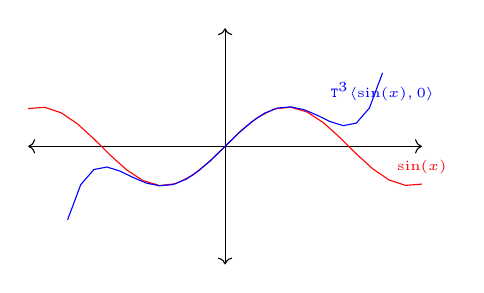
\begin{tikzpicture}[domain=-5:5, scale=0.5]
%\draw[very thin,color=gray] (-0.1,-1.1) grid (3.9,3.9);
\draw[<->]   (-5,0) -- (5,0);
\draw[<->] (0,-3) -- (0,3); % node[above] {$f(x)$};

   % \node at (0,0)[circle,fill,inner sep=1pt]{};
%
\draw[color=red, domain=-5:5] plot (\x, {sin(\x r) } ) node[above] {\tiny$\sin(x)$};

\draw[color=blue, domain=-4:4] plot (\x,{\x -((\x)^3)/6 + ((\x)^5/120  } ) node[below] {\tiny$\mathtt T^{3}\langle\sin(x),0\rangle$};


\end{tikzpicture}$}
}
\caption{\small The $\sup$-distance between $\sin(x)$ and its Taylor expansion $\mathtt T^{3}\langle\sin(x),0\rangle$ diverges.}
\label{fig:sintaylor}
\end{subfigure} \ \ \ 
\begin{subfigure}{0.45\textwidth}
\parbox[h][3.5cm][c]{\textwidth}{
\adjustbox{scale=0.55}{$
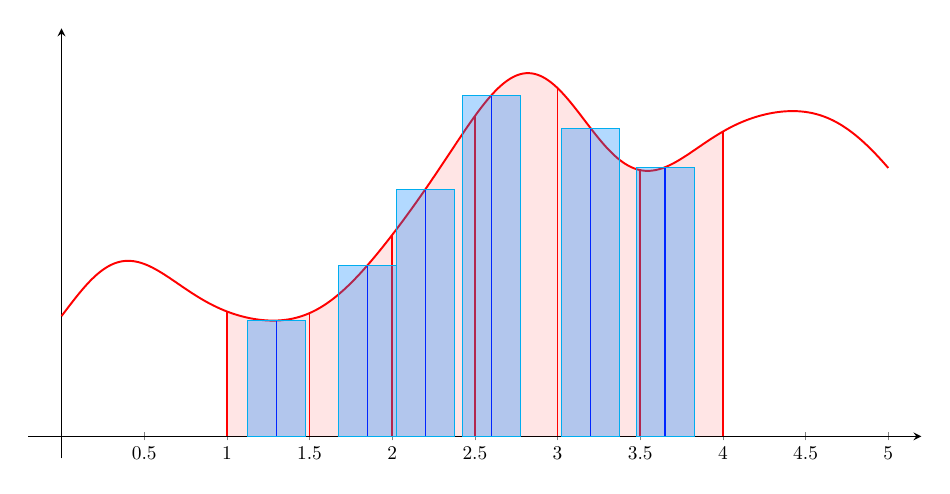
\begin{tikzpicture}[scale=0.7,
    declare function={
        f(\x)=2+sin(deg(\x-2))+sin(deg(3*\x))/2+sin(deg(5*\x))/8 + sin(deg(7*\x))/28;
    }
]
\begin{axis}[
    axis lines = middle,
    %xtick ={1,1.5,2,2.5,3,3.5,4},
    ytick ={0},
    %xticklabels = {$a=x_0$,$x_1$,$x_2$,$x_3$, $\ldots$, $x_{n-1}$,$x_n=b$},
    ymin = -0.2,
    ymax = 3.7,
    xmin = -0.2,
    xmax = 5.2,
    x=3cm,y=2cm,
    axis line style = thick,
    %xlabel={$x$},
    %ylabel={$y$},
    %extra x ticks={1.3,1.85,2.2,2.7,3.2,3.75},
%extra x tick labels={$\xi_1$, $\xi_2$, $\xi_3$, $\xi_4$, $\xi_{n-1}$, $\xi_n$},
]

\addplot [
    domain=1:4,
    samples=300,
    line width=1pt,
    fill=red, draw=none,
    fill opacity=0.1
] {f(x)} \closedcycle;

\addplot [
    domain=0:5,
    samples=300,
    line width = 1pt, red] {f(x)};

\addplot [
    ycomb, thick, red,
    no markers,
    samples at={1,1.5,...,4}
] {f(x)};

\addplot [
    ycomb, thick, blue,
    no markers,
    samples at={1.3,1.85,2.2,2.6,3.2,3.65}
] {f(x)};

\addplot[ybar, bar width=30pt, domain=1:4,
samples at={1.3,1.85,2.2,2.6,3.2,3.65}, fill=blue!50!cyan,fill opacity=0.3, draw=cyan]
  {f(x)};


\end{axis}
\end{tikzpicture}$}
}
\caption{\small Real integral $vs$ Riemann sum. \\ TO BE FIXED }
\label{fig:sintaylor}
\end{subfigure}
\end{figure}


\subparagraph*{Integral approximation}
A second natural example is numerical integration. Suppose that all functions in $\mathcal F_{n}$ are integrable and suppose we have at our disposal a term $\mathtt I_{r,s}: (\mathsf{Real}\to \mathsf{Real})\to \mathsf{Real}$ such that $\mathtt I_{r,s}f$ is (a precise enough approximation of) the definite integral $\int_{s}^{r}f(x)dx$.
In many contexts we might prefer to replace the expensive computation of $\mathsf I_{r,s}f$ by the (more economical but less precise) computation of a finite Riemann sum $\mathsf R^{n}_{r,s}f=  \sum_{i=1}^{n}(f x_{i})\cdot \Delta x$, where $\Delta x= |r-s|/n$ and $x_{i}= r+ i\cdot \Delta x$. 
It is well-known that the distance between the exact integral (that we suppose $\mathtt I_{r,s}$ is close enough to) and its approximation through a finite Riemann sum can be computed as a value $H(f'', n)$ depending on the second derivative of $f$ and $n$, that is
$d_{\mathsf{Real}}(\mathsf I_{r,s}f, \mathsf R^{n}_{r,s}f)\leq H(f'',n)$.

A bit more generally, we can consider the problem of bounding, given \emph{different} terms $f,g:\mathsf{Real}\to \mathsf{Real}$, the distance between the real integral of $\mathtt I_{r,s}f$ of $f$ and the approximate integral $\mathtt R^{n}_{r,s}g$ of $g$, supposing $f$ and $g$ are close each other on the interval $[r,s]$. 
 In fact, by standard calculation we can compute the bound
$d_{\mathsf{Real}} ( \mathsf{R}^{n}_{r,s}f, \mathsf R^{n}_{r,s}g)\leq 
d_{\mathsf{Real}\to\mathsf{Real}}(f, g)([r,s]) \cdot n (\Delta x)^{n}
$, which is small for small values of $|r-s|$. Then,
 using the triangular inequality we obtain an explicit bound
$d_{\mathsf{Real}} ( \mathsf{I}_{r,s}f, \mathsf R^{n}_{r,s}g)\leq
 d_{\mathsf{Real}} ( \mathsf{I}_{r,s}f, \mathsf R^{n}_{r,s}f)+
  d_{\mathsf{Real}} ( \mathsf{R}^{n}_{r,s}f, \mathsf R^{n}_{r,s}f)\leq 
 H(f'',n)+
d_{\mathsf{Real}\to\mathsf{Real}}(f, g)([r,s]) \cdot n (\Delta x)^{n}
$.

As in the previous example, we could not use the distance between $f$ and $g$ in a relevant way if this were the $\sup$-distance, since, although close on $[r,s]$, $f$ and $g$ might get arbitrarily far from each other over all reals. 



\subparagraph*{Loop perforation}
By adapting an example from \cite{chaudhuri}, we discuss a simplified example of the transformation which replaces $n$-iterations by $\lceil n/k \rceil$ iterations, in which only the iterations of $k\cdot i$ are performed and repeated $k$ times. 


Let $\mathsf{Nat}_{A}$ be a suitable type representing natural numbers in $\STLC$ and suppose  $t: (A\times A\to A) \to \mathsf{Nat}\to (A\to A)\to A$, for $n\geq 1$, is a term such that $th\mathtt n f$ 
computes the $n$-times iteration of $h$ as follows: $th \mathtt 0f= h\langle f\mathtt 0, f\mathtt 0\rangle$ and $th(\mathtt{n+1})f=h(th\mathtt n f, f\mathtt{n+1})$. 
Let $\mathsf{Perf}^{k}(t)$, the $k$-th perforation of $t$, be the function 
$\mathsf{Perf}^{k}(t)h\mathtt nf= t(\lambda x. (h^{(k)}x)) \mathtt{\lfloor n\rfloor_{k}} (\lambda x. f(x\cdot k)$, where $\lfloor n\rfloor_{k}$ indicates the least $m\leq n$ such that $m$ is divisible by $k$. 
It can then be checked that the distance 
$d_{A}(th\mathtt n f,  \mathsf{Perf}^{k}(t)h\mathtt nf  )$ between $t$ and its perforation can be bounded by 
computing the diameter of $\partial(t)   \partial(h) \tointerval{\mathtt n} (\lambda x.\partial (f)([\lfloor x/k\rfloor, x]))$.

%{
%
%given by $\mathsf{Perf}^{k}(t^{0})f= t^{0}f$ and $\mathsf{Perf}^{k}(t^{n+1})f=
%h( \mathsf{Perf}^{k}(t^{n})f, f \mathtt{\lfloor n+1/k\rfloor})$ if ${\lfloor n+1/k\rfloor}> {\lfloor n/k\rfloor}$, and $\mathsf{Perf}^{k}(t^{n+1})f=\mathsf{Perf}^{k}(t^{n})f$ otherwise.
%
%
%While $d_{A}(t^{1}f, \mathsf{Perf}^{k}(t^{1}f))$ is the self-distance of $t^{1}f\oeq_{\mathsf{A}}f\mathtt 0$ (which is equal to $0$ if, say, $A=\mathsf{Real}$), f

%
%
%As soon as we have a bound  $\rho: a,\mathtt n \mapsto \partial(h)(a,\tointerval{\mathtt n}) \vee a$
% for the smallest interval containing a value $t:A$ and its image $h(t,\mathtt n)$, we  can  compute explicit bounds for  the distance $d_{A}(t^{n}f,\mathsf{Perf}^{k}(t^{n})f)$. In fact, by letting $D_{A}(u,v): a\mapsto \tointerval u\vee \tointerval v$ and recalling that $d_{A}(u,v)=\diam_{A}(D_{A}(u,v))$, we can use the following lemma. 
%\begin{lemma}
%$D_{A}(t^{n+1}f, \mathsf{Perf}^{k}(t^{n+1})f)\leq H(n, \rho, \partial(h), \partial(f), D_{A}(t^{n}f,  \mathsf{Perf}^{k}(t^{n})f))$, where 
%%$\phi=d_{\mathsf{Real}\to \mathsf{Real}}(h,h)$, $\psi= d_{\mathsf{Real}\to \mathsf{Real}}(f,f) $ and , where $H(\phi,\psi,\Phi) $ is
%$H(n,\rho,\phi,\psi, \chi)=
%  \rho^{n}(\tointerval{f\mathtt 0})
%  +
%  \chi
%  +
% \psi( \chi, \psi (\mathtt{n+1},\mathtt{ \lfloor n+1/k\rfloor} ))
%$ and $\rho^{n}(a)$ is defined by $\rho^{0}(a)=a$ and $\rho^{n+1}(a)=\rho(\rho^{n}(a),\mathtt n)$.  
%%
%%In fact, since $t^{n+1}f= h \langle t^{n}f,  f\mathsf{n+1}  \rangle$ and 
%%$\mathsf{Perf}^{k}(t^{n+1})f$ is either equal to $\mathsf{Perf}^{k}(t^{n})f$, if $\lfloor n+1/k\rfloor=\lfloor n/k\rfloor$, or 
%%to $ h\langle \mathsf{Perf}^{k}(t^{n}f),  f\mathsf{\lfloor n+1/k\rfloor}  \rangle$, we have
%%$d_{A}(t^{n+1}f, \mathsf{Perf}^{k}(t^{n+1}f)) \leq d_{A}(t^{n+1}f, \mathsf{Perf}^{k}(t^{n}f)) +
%%d_{A\times A\to A}(h,h)( D_{A}( t^{n}f, \mathsf{Perf}^{k}(t^{n}f)),\partial(f)( a_{n,k}) )
%%$
%%where $a_{n,k}$ is the interval
%%$\big [ \mathtt{n+1},  \mathtt{\lfloor n+1/k\rfloor}\big ]_{A}$. 
%
%
%
%\end{lemma}
%\begin{proof}
%Computations are done in the appendix [ADD THEM].
%\end{proof}
%}
%






\section{Interval space models over a cartesian closed category}

% !TEX root = CSL 2021.tex
The examples from the last section relied on the fact that our partial metric semantics scales well to extensions of $\STLC$ with new base types and new program constructors. In this section we justify this fact in more general terms. In fact, we show that the constructions from Section \ref{section:stlc} can be reproduced starting from any model of the simply-typed $\lambda$-calculus. 


First, we need a suitable notion of model of the simply-typed $\lambda$-calculus to start with. Traditionally, one uses \emph{cartesian closed categories}: cartesian categories where, for all objects $A$, the functor $A \times -$ has a right adjoint (the \emph{exponential} functor). However, since many usual examples are in fact \emph{poset-enriched} categories (\textit{e.g.} Scott domains and continuous functions, coherent spaces and stable functions), and since any (locally small) category can be poset-enriched by using equality as the ordering, we will consider instead \emph{cartesian closed poset-enriched categories}. To give a counterpart to Proposition \ref{prop:intervals-weak-model-lambda}, we also need a notion of ``weak'' model of the simply-typed $\lambda$-calculus: since poset-enriched categories are a particular case of $2$-categories (with a unique $2$-arrow from $f$ to $g$ if and only if $f \leq g$), we follow Hilken \cite{hilken:2-lambda} and consider cartesian categories where, for all objects $A$, the functor $A \times -$ has a lax right adjoint (the \emph{lax-exponential} functor).

Products and exponentials, when they exist, are necessarily unique up to unique isomorphism: thus, traditionally, a cartesian closed category is defined as a category in which all finite products and exponentials exist, rather than a category \emph{equipped} with products and exponentials (\textit{i.e.} it is a category with a given \emph{property}, rather than a category with additional \emph{structure}). However, this is not the case for lax-exponentials, so for consistency we will adopt the ``structure'' picture in both cases. Adapting Hilken's definitions \cite{hilken:2-lambda} to the simpler case of poset-enriched categories, we obtain:

\begin{definition} Let $(\mathbb{C}, \times, 1)$ be a cartesian poset-enriched category. An \emph{exponential} (respectively, a \emph{lax-exponential}) on $\mathbb{C}$ is the data of a map $\exp$ from $\operatorname{Ob}(\mathbb{C} \times \mathbb{C})$ to $\operatorname{Ob}(\mathbb{C})$ and two families of monotone maps $(\ev_{W,X,Y} : \mathbb{C}(W, \operatorname{exp}(X,Y)) \to \mathbb{C}(W \times X, Y))$ and $(\lam_{W,X,Y} : \mathbb{C}(W \times X, Y) \to \mathbb{C}(W, \exp(X,Y)))$ such that: \begin{itemize}
\item $\ev_{W,X,Y}$ and $\lambda_{W,X,Y}$ are natural with respect to $W$,
\item for all $g \in \mathbb{C}(W \times X, Y)$, $\ev(\lam(g)) = g$ (respectively, $\ev(\lam(g)) \leq g$),
\item for all $f \in \mathbb{C}(W, \exp(X,Y))$, $f = \lam(\ev(f))$ (respectively, $f \leq \lambda(\operatorname{ev}(f))$).
\end{itemize}
\end{definition}

One can check that this definition makes $\exp$ a functor (respectively, a lax-functor) from $\operatorname{Ob}(\mathbb{C}^{\operatorname{op}} \times \mathbb{C})$ to $\operatorname{Ob}(\mathbb{C})$ (with
$\exp(f,g)$ defined as $\lam(g\circ\ev(\id)\circ(\id\times f))$). In addition, this definition implies that $\ev$ and $\lam$ are natural, in the sense that $\ev(\exp(\alpha,\beta)\circ f\circ\gamma) = \beta\circ\ev(f)\circ(\gamma\times\alpha)$ and $\exp(\alpha,\beta)\circ\lam(g)\circ\gamma = \lam(\beta\circ g\circ(\gamma\times\alpha))$ (respectively, lax-natural \cite{hilken:2-lambda}, in the sense that $\ev(\exp(\alpha,\beta)\circ f\circ\gamma) \leq \beta\circ\ev(f)\circ(\gamma\times\alpha)$ and $\exp(\alpha,\beta)\circ\lam(g)\circ\gamma \leq \lam(\beta\circ g\circ(\gamma\times\alpha))$).

For the rest of this section, we fix a cartesian poset-enriched category $(\mathbb{C}, \times, 1)$ (we denote by $\langle-,-\rangle$ the pairing transformation and by $\pi_L$ and $\pi_R$ the projections) and an exponential $(\exp, \ev, \lam)$ on $\mathbb{C}$. The morphisms of this category represent \emph{exact programs}, so they play the role of the terms from Section \ref{section:stlc}.

\begin{definition} A \emph{$\mathbb{C}$-diameter space} $A$ is the data of \begin{itemize}
\item an object $\bs{A}$ of $\mathbb{C}$. The poset $\mathbb{C}(1,\bs{A})$ will be denoted by $\Lambda_A$;
\item a set $\intervals{A}$ of downwards-closed subsets of $\Lambda_A$ that is closed under arbitrary intersections. In particular, $\intervals{A}$ is a complete lattice whose meet is given by intersection, and for all $t\in\Lambda_A$, there is a least element of $\intervals{A}$ that contains $t$, which will be denoted by $\tointerval{t}$;
\item a commutative integral quantale $(\distances{A}, \quantaleop, \quantalegeq)$;
\item a monotone function $\diam_A : \intervals{A} \to \distances{A}$ such that $$\forall a,b \in \intervals{A} \text{ s.t. } a \wedge b \neq \emptyset,~ \diam(a \wedge b) \quantaleop \diam(a \vee b) \quantalegeq \diam(a) \quantaleop \diam(b)\text{,}$$
and such that for all $t,u \in \Lambda_A$, if $\diam_A(\tointerval{t}) = \diam_A(\tointerval{t} \vee \tointerval{u})$, then $\tointerval{t} = \tointerval{t} \vee \tointerval{u}$.
\end{itemize}
\end{definition}

The role of the condition $a \wedge b \neq \emptyset$ is illustrated by Fig. \ref{fig:modular}.

\begin{example} If $\mathbb{C}$ is the category whose objects are the simple types from Section \ref{section:stlc} and whose morphisms are the (open) terms modulo $\beta$-equivalence, then for all simple types $A$, $(A, \intervals{A}, \distances{A}, \diam_A)$ defines a $\mathbb{C}$-diameter space.
\end{example}

Following Section \ref{section:stlc}, for all $\mathbb{C}$-diameter spaces $A$ and $B$, we define a $\mathbb{C}$-diameter space $A \times B$ such that $\bs{A \times B} = \bs{A} \times \bs{B}$ and a $\mathbb{C}$-diameter space $\exp(A,B)$ such that $\bs{\exp(A,B)} = \exp(\bs{A},\bs{B})$: \begin{itemize}
\item $\intervals{A \times B} = \{ a \times b \mid a \in \intervals{A}, b \in \intervals{B} \} $, where $a \times b = \{ t \in \mathbb{C}(1, \bs{A} \times \bs{B}) \mid \pi_L \circ t \in a \text{ and } \pi_R \circ t \in b \}$,
\item $\distances{A \times B} = \distances{A} \times \distances{B}$,
\item $\diam_{A \times B}(c) = (\diam_A(\{ \pi_L \circ t \mid t \in c \}), \diam_B(\{ \pi_R \circ t \mid t \in c \}))$,
\item $\intervals{\exp(A, B)} = \{ \{ t \in \mathbb{C}(1, \exp(\bs{A}, \bs{B})) \mid \forall u \in \Lambda_{A},~ \ev(t) \circ u \in I(u) \} \mid I\in \operatorname{Poset}(\Lambda_A, \intervals{B}) \}$,
\item $\distances{\exp(A, B)} = \operatorname{Poset}(\intervals{A}, \distances{B})$,
\item $\diam_\mathsf{\exp(A, B)}(c) = a \mapsto \diam_B\left(\sup\left\{\tointerval{\ev(v) \circ t} \mid t\in a, v \in c\right\}\right).$
\end{itemize}

We need a counterpart to Proposition \ref{prop:intervals-weak-model-lambda}. As explained above, we obtain this by organizing the $\mathbb{C}$-diameter spaces as a cartesian poset-enriched category with a lax-exponential. First, we need to define a notion of morphisms between two $\mathbb{C}$-diameter spaces $A$ and $B$ (which represent \emph{approximate programs}). By analogy with Section \ref{section:stlc}, these will be monotone functions from $\intervals{A}$ to $\intervals{B}$; however, in order to actually obtain a cartesian category (which was not an issue in Section \ref{section:stlc}), we will need to add an extra condition:

\begin{definition}
We denote by $\dsp(\mathbb{C})$ the poset-enriched category defined as follows: \begin{itemize}
\item the objects of $\dsp(\mathbb{C})$ are the $\mathbb{C}$-diameter spaces,
\item for all $\mathbb{C}$-diameter spaces $A$ and $B$, $\dsp(\mathbb{C})(A,B)$ is the set of all monotone functions $\varphi : \intervals{A} \to \intervals{B}$ such that there exists $f \in \mathbb{C}(\bs{A},\bs{B})$ such that for all $t \in \Lambda_A$, $f \circ t \in \varphi\left(\tointerval{t}\right)$ (ordered by pointwise inclusion).
\end{itemize}
\end{definition}

One can check that the operation $-\times-$ defined above on $\mathbb{C}$-diameter spaces is a cartesian product in $\dsp(\mathbb{C})$. In addition, one can check that there exists in $\dsp(\mathbb{C})$ a terminal object $1_{\dsp(\mathbb{C})}$ such that $\bs{1_{\dsp(\mathbb{C})}} = 1_{\mathbb{C}}$. In other words, $\dsp(\mathbb{C})$ is cartesian. Here too, we denote by $\langle-,-\rangle$ the pairing transformation and by $\pi_L$ and $\pi_R$ the projections.


Now, following Section \ref{section:stlc}, we can complete the definition of the lax-exponential: let $A,B,C$ be $\mathbb{C}$-diameter spaces, \begin{itemize}
\item for all $\varphi \in \dsp(\mathbb{C})(A, \exp(B, C))$, we define $\ev_{A,B,C}(\varphi) \in \dsp(\mathbb{C})\allowbreak(A \times B, C)$ by $\ev_{A,B,C}(\varphi)(p) = \sup\left\{ \tointerval{\ev(v) \circ u} \mid v \in \varphi(\pi_L(p)), u \in \pi_R(p) \right\}$,
\item for all $\psi \in \dsp(\mathbb{C})(A \times B, C)$, we define $\lam_{A,B,C}(\psi) \in \dsp(\mathbb{C})(A,\allowbreak \exp(B, C))$ by $\lam_{A,B,C}(\psi)(a) = \{ v \in \Lambda_{\exp(B, C)} \mid \forall u \in \Lambda_B,~ \ev(v) \circ u \in \psi(a \times \tointerval{u}) \}$.
\end{itemize}
 
 \begin{proposition} The triple $(\exp, \ev, \lam)$ is a lax-exponential on $\dsp(\mathbb{C})$.
 \end{proposition}
 \begin{proof} Naturality with respect to $A$ is immediate.
 
Let $p = a \times b \in \intervals{A \times B}$. For all $v \in \lam(\psi)(a)$ and and $u \in b$, by definition $\ev(u) \circ u \in \psi(a \times \tointerval{u}) \subseteq \psi(p)$. Therefore, $\ev(\lam(\psi))(p) \subseteq p$.
 
 Let $a \in \intervals{A}$ and $v \in \varphi(a)$. For all $u \in \Lambda_B$,  by definition, $\ev(v) \circ u \in \lambda(\varphi)(a \times \tointerval{u})$, so $v \in \lam(\ev(\varphi))(a)$.
\end{proof}
 
As in Section \ref{section:stlc}, we can find a kind of weak embedding from $\mathbb{C}$ to $\dsp(\mathbb{C})$. Namely, for all $\mathbb{C}$-diameter spaces $A$ and $B$, we define a monotone map $\partial : \mathbb{C}(\bs{A}, \bs{B}) \to \dsp\allowbreak(\mathbb{C})(A, B)$ by $\partial(f)(a) = \sup \{ \tointerval{f \circ t} \mid t \in a \}$. The following compatibility result is immediate and offers a counterpart to Remark \ref{remark:oplax-functor-stlc}:

\begin{proposition} For all $\mathbb{C}$-diameter spaces $A, B, C$, all $f \in \mathbb{C}(A, B)$ and all $g \in \mathbb{C}(B, C)$, $\partial(g \circ f) \leq \partial(g) \circ \partial(f)$. In addition, $\partial(\operatorname{id}_{\bs{A}}) = \operatorname{id}_A$.
\end{proposition}
 
One way to reformulate this result is that $\partial$ induces an oplax-functor from the category with the same objects as $\dsp(\mathbb{C})$ and the same morphisms as $\mathbb{C}$, to $\dsp(\mathbb{C})$.

One can check that $\partial$ preserves products, in the sense that $\partial (\langle f, g \rangle) = \langle\partial(f), \partial(g)\rangle$, $\partial(\pi_L) = \pi_L$ and $\partial(\pi_R) = \pi_R$. In addition $\partial$ is weakly compatible with the exponential, which corresponds to Remark \ref{remark:push-exp-stlc}:

\begin{proposition} Let $A, B, C$ be $\mathbb{C}$-diameter spaces, \begin{itemize}
\item for all $f \in \mathbb{C}(\bs{A}, \exp(\bs{B}, \bs{C}))$, $\partial(\ev(f)) \leq \ev(\partial(f))$,
\item for all $g \in \mathbb{C}(\bs{A}\times\bs{B}, \bs{C})$, $\partial(\lam(g)) \leq \lam(\partial(g))$.
\end{itemize}
\end{proposition}

Finally, following Section \ref{section:stlc}, for all $\mathbb{C}$-diameter spaces $A$ and all  $t,u \in \Lambda_A$, we write $t \oeq_A u$ if $\tointerval{t} = \tointerval{u}$. In addition, we define a function $d_A : \Lambda_A \times \Lambda_A \to \distances{A}$ by $d_A(t,u) = \diam_A(\tointerval{t} \vee \tointerval{u})$. Then the same arguments as in Corollary \ref{corollary:stlc-metric} show that:

\begin{proposition} For all $\mathbb{C}$-diameter spaces $A$, \emph{$(\Lambda_{A}/\oeq_{A}, \distances{A}, d_{A})$ is a generalized partial metric space}.
\end{proposition}

One can check that what is described in Section \ref{section:stlc} is indeed an instance of this construction. Here are a couple more examples:

\begin{example} We can take $\mathbb{C} = \set$ (with the morphisms ordered by equality): $\dsp(\set)$ contains an object $\mathsf{Real}_{\set}$ that represents the real numbers with their standard metric and the compact intervals (plus $\emptyset$ and $\mathbb{R}$) as approximate values, namely $\bs{\mathsf{Real}_{\set}} = \mathbb{R}$, $\intervals{\mathsf{Real}_{\set}} = \{ \text{the compact intervals}, \emptyset, \mathbb{R} \}$, $\distances{\mathsf{Real}_{\set}} = [0,\infty]$ and $\diam_{\mathsf{Real}_{\set}}(I) = \operatorname{length}(I)$.

In this case, $\bs{\exp(\mathsf{Real}_{\set}, \mathsf{Real}_{\set})}$ is the set of all functions from $\mathbb{R}$ to $\mathbb{R}$, so $d_{\mathsf{Real}_{\set}}$ defines a partial metric on all such functions.
\end{example}

\begin{example} We can take $\mathbb{C} = \eff$, the effective topos \cite{hyland:effective-topos}: $\eff$ contains an object $\mathbb{R}_{\eff}$ of recursive reals, and we can define an object $\mathsf{Real}_{\eff}$ in $\dsp(\eff)$ by $\bs{\mathsf{Real}_{\eff}} = \mathbb{R}_{\eff}$, $\intervals{\mathsf{Real}_{\eff}} = \{ I \cap \mathbb{R}_{\eff} \mid I \in \intervals{\mathsf{Real}_{\set}} \}$, $\distances{\mathsf{Real}_{\eff}} = [0,\infty]$ and $\diam_{\mathsf{Real}_{\eff}}(I) = \operatorname{length}(I)$.

In this case, $\bs{\exp(\mathsf{Real}_{\eff}, \mathsf{Real}_{\eff})}$ is the set of all recursive functions from $\mathsf{Real}_{\eff}$ to $\mathsf{Real}_{\eff}$, so $d_{\mathsf{Real}_{\eff}}$ defines a partial metric on all such functions.
\end{example}

\begin{example} We can take $\mathbb{C} = \scott$, the poset-enriched category of Scott domains and continuous functions. It contains an object representing the reals: $\mathbb{R}_{\scott} = (\mathbb{R} \cup \{ \bot \}, \sqsubseteq)$, with $r \sqsubseteq s$ \textit{iff} $r = s$ or $r = \bot$. Again, we can define in  $\dsp(\scott)$ an object $\mathsf{Real}_{\scott}$ that represents the real numbers with their standard metric, and this defines a partial metric on $\bs{\exp(\mathsf{Real}_{\scott}, \mathsf{Real}_{\scott})}$, the set of all Scott continuous functions from $\mathbb{R}_{\scott}$ to $\mathbb{R}_{\scott}$, which are essentially the partial functions from $\mathbb{R}$ to $\mathbb{R}$.
\end{example}

 

\section{Related work}

% !TEX root = CSL 2021.tex

 

\begin{figure}
\begin{subfigure}{0.45\textwidth}
\parbox[h][4.6cm][c]{\textwidth}{
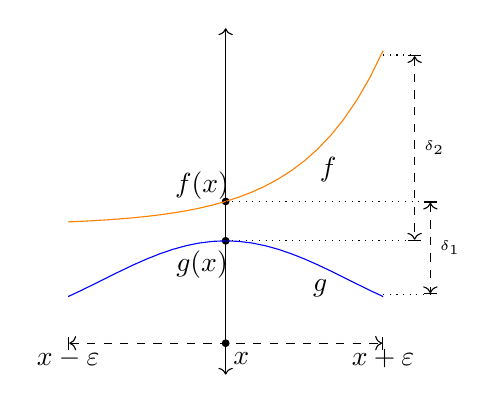
\begin{tikzpicture}[domain=-2:2]
%\draw[very thin,color=gray] (-0.1,-1.1) grid (3.9,3.9);
\draw[dashed, |<->|]   (-2,0) -- (2,0);
\draw[<->] (0,-0.4) -- (0,4); % node[above] {$f(x)$};

    \node at (0,0)[circle,fill,inner sep=1pt]{};
%    \node at (-2,0)[circle,fill,inner sep=1pt]{};
%    \node at (2,0)[circle,fill,inner sep=1pt]{};
\node(z) at (0.2,-0.2) {$x$};
\node(-e) at (-2,-0.2) {$x-\varepsilon$};
\node(e) at (2,-0.2) {$x+\varepsilon$};


\node(f) at (0,0.8+0.5)[circle,fill,inner sep=1pt]{};
\node(f) at (0,1.5+0.3)[circle,fill,inner sep=1pt]{};

\node(f) at (-0.3,2) {$f(x)$};

\node(f) at (-0.3,1) {$g(x)$};


\node(ff) at (1.3,2.2) {{$f$}};
\node(gg) at (1.2,0.7) {{$g$}};

%\draw[color=red] plot (\x,\x) node[right] {$f(x) =x$};
% \x r means to convert ?\x? from degrees to _r_adians:
\draw[color=blue] plot (\x,{0.8+ 0.5*(cos(\x r))}) ;
\draw[color=orange] plot (\x,{1.5+0.3*exp(\x)}) ;

\draw[dotted] (0,1.8) -- (2.6,1.8);
\draw[dotted] (2,0.62) -- (2.6,0.62);
\draw[dotted] (0,1.3) -- (2.4,1.3);
\draw[dotted] (2,3.66) -- (2.4,3.66);

%
%\draw[dotted] (0,1.8) -- (2, 0.62);
%\draw[dotted] (0,1.3) -- (2, 3.66);

\draw[dashed,|<->| ] (2.4,3.66) -- node[right] {\tiny$\delta_{2}$} (2.4,1.3);
\draw[dashed,|<->| ] (2.6,1.8) -- node[right] {\tiny$\delta_{1}$} (2.6,0.62);

\end{tikzpicture}
}
\caption{\small In differential logical relations the distance between two functions $f,g:\R\to \R$, computed at $(x,\varepsilon)$ is the maximum between 
$\delta_{1}=\max\{d(f(x),g(y));~ y\in [x-\varepsilon, x+\varepsilon]\}$ and 
$\delta_{2}=\max\{d(g(x), f(y));~ y\in [x-\varepsilon, x+\varepsilon]\}$.}
% and 
%
%
%minimum $\delta$ such that for all $y\in [x-\varepsilon, x+\varepsilon]$, both $g(y)\in [f(x)-\delta, f(x)+\delta]$ and $f(y)\in[g(x)-\delta, g(x)+\delta]$ hold. $\delta$ is thus $\max\{\delta_{1},\delta_{2}\}$ in the image above.}
\label{fig:graph1}
\end{subfigure} \ \ \ \ 
\begin{subfigure}{0.45\textwidth}
\parbox[h][4.6cm][c]{\textwidth}{
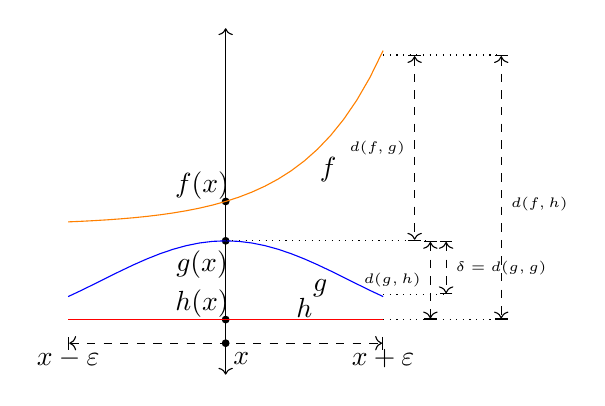
\begin{tikzpicture}[domain=-2:2]
%\draw[very thin,color=gray] (-0.1,-1.1) grid (3.9,3.9);
\draw[dashed, |<->|]   (-2,0) -- (2,0);
\draw[<->] (0,-0.4) -- (0,4); % node[above] {$f(x)$};

    \node at (0,0)[circle,fill,inner sep=1pt]{};
%    \node at (-2,0)[circle,fill,inner sep=1pt]{};
%    \node at (2,0)[circle,fill,inner sep=1pt]{};
\node(z) at (0.2,-0.2) {$x$};
\node(-e) at (-2,-0.2) {$x-\varepsilon$};
\node(e) at (2,-0.2) {$x+\varepsilon$};


\node(f) at (0,0.8+0.5)[circle,fill,inner sep=1pt]{};
\node(f) at (0,1.5+0.3)[circle,fill,inner sep=1pt]{};
\node(f) at (0,0.3)[circle,fill,inner sep=1pt]{};

\node(f) at (-0.3,2) {$f(x)$};

\node(f) at (-0.3,1) {$g(x)$};

\node(f) at (-0.3,0.5) {$h(x)$};

\node(ff) at (1.3,2.2) {{$f$}};
\node(gg) at (1.2,0.7) {{$g$}};
\node(gg) at (1,0.45) {{$h$}};

%\draw[color=red] plot (\x,\x) node[right] {$f(x) =x$};
% \x r means to convert ?\x? from degrees to _r_adians:
\draw[color=blue] plot (\x,{0.8+ 0.5*(cos(\x r))}) ;
\draw[color=orange] plot (\x,{1.5+0.3*exp(\x)}) ;
\draw[color=red] plot (\x,{0.3}) ;



\draw[dotted] (0,1.3) -- (2.6,1.3);
\draw[dotted] (2,0.3) -- (3.5,0.3);
\draw[dotted] (0,1.3) -- (2.4,1.3);
\draw[dotted] (2,3.66) -- (3.5,3.66);
\draw[dotted] (2,0.62) -- (2.8,0.62);

%
%\draw[dotted] (0,1.8) -- (2, 0.62);
%\draw[dotted] (0,1.3) -- (2, 3.66);

\draw[dashed,|<->| ] (2.4,3.66) -- node[left] {\tiny$d(f,g)$} (2.4,1.3);
\draw[dashed,|<->| ] (2.6,1.3) -- node[left] {\tiny$d(g,h)$} (2.6,0.3);

\draw[dashed,|<->| ] (2.8,1.3) -- node[right] {\tiny$\delta=d(g,g)$} (2.8,0.62);

%\draw[dashed,|<->| ] (3.5,2.96) -- node[above right] {\tiny$\begin{matrix}d(f,g)+d(g,h)\\ -d(g,g)\end{matrix}$} (3.5,0.3);

\draw[dashed,|<->| ] (3.5,3.66) -- node[below right] {\tiny$d(f,h)$} (3.5,0.3);

\end{tikzpicture}
}
%
\caption{\small The distance arising from differential logical relations is not a partial metric: the example above shows that $d(f,h)> d(f,g)+d(g,h)- d(g,g)$ (with all distances computed in $(x,\varepsilon)$).}% and 
%
%
%minimum $\delta$ such that for all $y\in [x-\varepsilon, x+\varepsilon]$, both $g(y)\in [f(x)-\delta, f(x)+\delta]$ and $f(y)\in[g(x)-\delta, g(x)+\delta]$ hold. $\delta$ is thus $\max\{\delta_{1},\delta_{2}\}$ in the image above.}
\label{fig:graph2}
\end{subfigure}
\end{figure}

\subparagraph*{Related work}


A primary source of inspiration for our approach was the recent work of Dal Lago, Gavazzo and Yoshimizu on  \emph{differential logical relations} \cite{dallago:differential-stlc}. This is a semantics for higher-order languages in which a type is interpreted as a set $X$ endowed with a kind of metric structure expressed by a relation $\rho \subseteq X\times \mathbb Q\times X$, where $\mathbb Q$ is an arbitrary quantale. To our knowledge, this is the first place were the idea of varying the quantales in which distances are measured is introduced as a key ingredient to obtain a cartesian closed category.

While the relation $\rho$ of a GMS induces a distance function $d_{\rho}(x,y)=\sup\{\epsilon\mid \rho(x,\epsilon,y)\}$, this function is not a partial metric. We can show this fact with a simple example: in this model the distance between two programs 
 $f,g:\mathsf{Real}\to \mathsf{Real}$ is taken in the quantale of functions from $\R\times \R_{+}^{\infty}$ to $\R_{+}^{\infty}$: intuitively, 
  $d(f,g)$ associates a closed interval $[x-\epsilon,x+\epsilon]$ (corresponding to the pair $(x,\varepsilon)$) with the smallest distance $\delta$ such that $[ f(x)-\delta, f(x)+\delta]$ and $[g(x)-\delta,g(x)+\delta]$ both contain the images of $[x-\varepsilon, x+\varepsilon]$ through
 $g$ and $f$ respectively (see Fig. \ref{fig:graph1}). Then, as shown in Fig. \ref{fig:graph2}, by letting $\delta=d(g,g)(x,\varepsilon)$, we have that $d(g,g)$ sends the interval $I=[x-\varepsilon, x+\varepsilon]$ onto the interval $[g(x)-\delta, g(x)+\delta]$, which has diameter $2\delta$, while the image of $I$ has diameter $\delta$, making the triangular law of partial metrics fail. 



A more syntactic approach to approximate program transformations is the one in 
\cite{chaudhuri}, which introduces a System F-based type system with a type of real numbers and an explicit distinction between exact and approximate programs.
%, and provides typing rules to formalize contextual reasoning about program differences. As in the case of differential logical relations, program differences are taken as functions relating errors in input and errors in output, but the viewpoint of program metric is not considered.
Like the case of loop perforation discussed in Section 4, most examples of contextual reasoning from \cite{chaudhuri} can be  reformulated in our framework. 




The literature on program pseudo-metrics is vast. A major distinction can be made between those approaches in which metrics account for \emph{extensional} aspects of programs (like ours), 
 and approaches in which metrics are used to characterize \emph{intensional} aspects.
To the first family belong all metric models developed for reasoning about differential privacy \cite{},  
probabilistic computation \cite{} and co-inductive models \cite{}.
%In particular, several approaches like \cite{} emphasize the importance to formalize contextual reasoning, wich can be assured in frameworks like \cite{} by the restriction to Lipschitz-continuous or non-expansive functions. 
To the second class belong approaches like \cite{} which recovers the Scott model of PCF through a ultrametric semantics, as well as most of previous models based on partial metric spaces, which rely on a correspondence between continuous Scott domains and the $T_{1}$ topology of partial metrics.
%
%. 
%The central motivation such approaches is the observation that a partial metric $d$ on a set $X$ induces an order relation given by $x\preceq_{d}y$ iff $d(x,y)\leq d(x,x)$, turning $X$ into a continuous Scott domain and, conversely, any continuous Scott domain with a countable basis is induced by a partial metric in this way.
%This allows to reformulate several classical results on denotational semantics using the $T_{1}$ topology of partial metric spaces.
%


More recently, \cite{Stubbe} introduced an elegant categorical approach to GPMS in the framework of \emph{quantaloid-enriched categories}, as well as a 
characterization of exponentiable GPMS, showing in particular that no such category can be both cartesian closed categories and contain the standard metric on $\mathbb R$. This result seems to add further evidence of the necessity of considering metrics over varying quantales in order to model higher-order languages. 
%
%While in all these results distances are computed over a \emph{fixed} quantale, the generalization of this categorical approach to varying quantales seems to be a yet unexplored research direction.






\subparagraph*{Future work}


%
%
%In this paper we constructed a (non-extensional) model of the simply typed $\lambda$-calculus based on generalized partial metric spaces. Our model provides a 
% differential semantics of higher-order programs, that is, a semantic description of \emph{differences} between
% higher-order programs. 
% The main novelty is that we take as morphisms between metric spaces approximate functions, \emph{i.e.} monotone functions over intervals, rather than continuous functions of some kind. While approximate functions represent sets of similar programs, usual, exact, programs can be embedded in the model through a differentiation operator. 
% This approach allows us to overcome the well-known obstacle that usual categories of metric spaces and continuous functions are not cartesian closed, and therefore cannot be models of $\STLC$.
%% 
% Instead, we obtain 
%based on generalized partial metric spaces and
%
%Moreover, our model refines previous notions of program distances based on differential logical relations.
%
%
%the use of partial metric spaces, a well-investigated metric structure to which most fundamental properties and results on standard metric spaces scale well, 
%
%
%
%
%. More importantly, we take, as morphisms between them, approximate functions, that is, function over closed intervals, rather than (Lipschitz-) continuous or non-expansive functions over points, as in usual categories of metric spaces.

The approach we presented lends itself to further extensions and generalizations.
First, we would like to investigate the interpretation of more type constructions than those of $\STLC$ (e.g. sum types, recursive types, effects). Moreover, we would like to explore the possibility of exploiting the structure of the category $\dsp(\mathbb C)$ to construct new and more refined notions of approximations.
For example (we work in $\dsp(\set))$ for simplicity), 
starting from the ``standard'' set of approximate values $\mathcal I$ on $\mathbb{R}^{X\times X}$ (with elements of $\mathcal I$ being  families of compact intervals $U_{x,x'}\subseteq \mathbb R$ indexed by values in $X\times X$), one can define a new family  $\Delta^{*}\mathcal I$  of approximate values for  $\mathbb R^{X}$ by ``pulling back'' the exact map 
$\Delta:
\mathbb R^{X} \to \mathbb R^{X\times X}$ defined by $\Delta f(x,x')=f(x')-f(x)$. 
The new approximate values corresponds then to sets of functions $f\in \mathbb R^{X}$ with a controlled variation, that is, such that $f(x')-f(x)$ is bounded by some family of intervals $U_{x,x'} \in \mathcal I$.





%
%First, in this paper we restricted our attention to $\STLC$, which is not a universal language. 
%The accommodation of full recursion in metric models is usually obtained by an application of the Banach fixed point theorem \cite{VANBREUGEL20011}. As this theorem scales well to partial metric spaces \cite{Samet:2013aa}, a natural question is whether our model, or some variant of it, can be used to provide a metric account of universal computation over the real numbers.
%


Another interesting research direction concerns probabilistic extensions of $\STLC$. 
Probabilistic metrics \cite{1029849,KOZEN1981328, 10.1109/LICS.2015.64, 10.1007/978-3-662-54434-1_13} have been the object of much research in recent years, due to the relevance of metric reasoning in some areas of computer science in which probabilistic computation plays a key role (e.g. in cryptography \cite{GOLDWASSER1984270} and machine learning \cite{krause08robust}).
A convenient starting point seems to be the recent generalization of {probabilistic (generalized) metric spaces} to the partial metric case \cite{HE201999}.






\section{Conclusions}

\input{conclusions}

\bibliography{CSL2021.bib}


\appendix

\section{Generalized partial metric spaces}

\input{partialmetricspaces}

\section{Cartesian lax-closed categories}

\input{cclaxc}
\end{document}
